\documentclass[main.tex]{subfiles}
\begin{document}

\chapter{NEMO detectors}


\NI Initiated in the late 1980s, the main aim of the NEMO project is the search for 0$\nu\beta\beta$. The strategy adopted by the collaboration is the direct detection of the 2 electrons emitted in $\beta\beta$ decay. A strategic point in the search for these very rare processes is the background level. The detectors must be installed in underground laboratory to be protected from the cosmic rays but also all the materials enter in the detector fabrication have to be radiopure.


\bigskip


\NI This chapter presents the different phases and the different prototypes built by the NEMO collaboration. The principe of the NEMO detection is presented in Section~\ref{sec:Principe}. Section~\ref{sec:LSM} shortly describes the Modane undergound laboratory where the NEMO detectors were hosted. The 2 first prototypes NEMO-1 and NEMO-2 are presented in Section~\ref{sec:NEMO1-2}. Section~\ref{sec:NEMO3} and \ref{sec:SuperNEMO} describe respectively the NEMO-3 detector and the SuperNEMO project.


\section{Historical and principle}


\subsection{Principe}\label{sec:Principe}


To directly detect the 2 electrons emitted in $\beta\beta$ decay, the $\beta\beta$ sources consist of thin foils placed at the center of the detector and surrounded by a tracking device for electron track reconstruction. The tracking volume is itself surrounded by a calorimeter for electron energy measurement. Figure~\ref{SchemaNEMOl} presents the detection principle of $\beta\beta$ event combining tracking and calorimetric measurements. This unique feature allow a full reconstruction of the different parameters of the events. The energy of each particle can be measured independently also as the angles between the particle tracks, which allows the discrimation between the processes behind $\beta\beta$ decay and a good background discrimination. Futhermore, this approach permits to search for the 0$\nu\beta\beta$ decays among several isotopes. 


\begin{figure}[h!]
\begin{center}
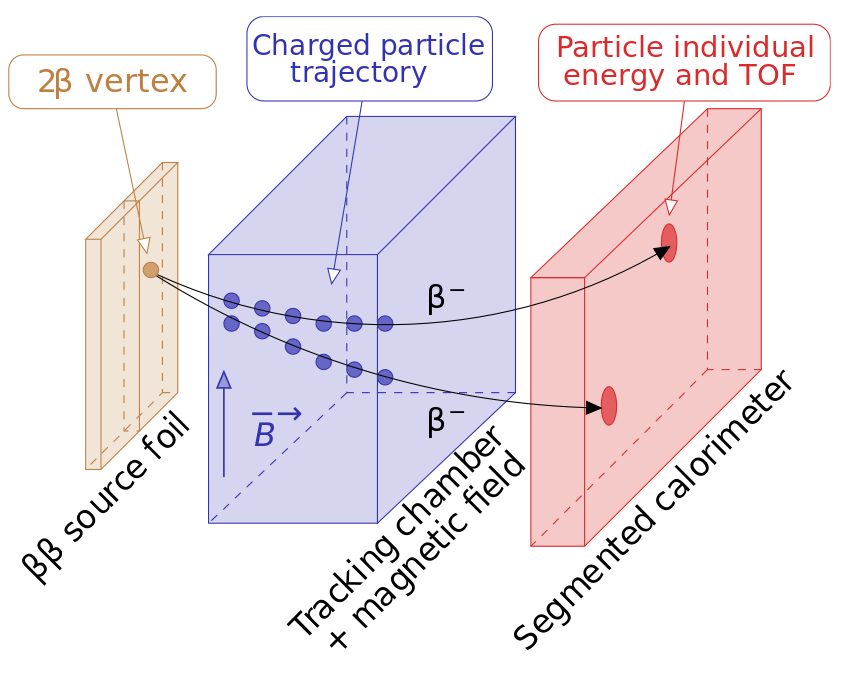
\includegraphics[scale=0.30]{pictures/Chap3/SchemaNEMO.png}
\caption{Detection principe of a $\beta\beta$ event combining tracking and calorimetric measurement. A thin $\beta\beta$ source is placed at the center of the detector. A tracking chamber allied with a magnetic field reconstruct the particle trajectory. The particle energy and their time of fligh is obtained with a calorimeter.}
\label{SchemaNEMOl}
\end{center}
\end{figure}


\subsubsection{$\beta\beta$ source foils}


\NI The $\beta\beta$ source foils of the NEMO project are the central part of the detectors. They can be metallic or composite but in anycase a great care is taken in their fabrication, and more particularly about their radio-purity. The foils must be the thinest as possible to avoid energy loss of the leaving particles. On the other hand, they have to be strong enough to withstand all the time of the experiment. More details about the source foils and their fabrication will be given in the next sections.


\subsubsection{Tracking volume}


\NI The tracking device of the NEMO experiments is a wire chamber working in Geiger mode coupled with a magnetic field for charge discrimination. Each Geiger cell is composed by a central wire (called anode) and surrunded by 8 wires distributed on an circle (cathode), a voltage difference is applied between the cathode and the anode.


\bigskip


\NI When a charged particle crosses the tracking volume, the gas is ionized by photoelectric effect. Due to the high voltage, the created electrons will migrate to the anode and be multiplied in a avalanche. Some photons are also emitted and generate other avalanches, this chain reaction is called Townsend avalanche, shown in Figure~\ref{avalancheTownsend}. For a short time, the gas is conductive, and the plasma propagates along both side of the anodic wire. The arrival time of the plasma at the endcaps provides informations on the longitudinal distance of the particle interaction point. The radial position to the anode is determine by the drift time (in this case a trigger is necessary which is given by the calorimeter). By knowing the longitudinal and radial distance of several Geiger cells, the particle 3-D track can be reconstructed. The discharge ends when the positive ions concentration is high enough to counterbalance the electric field. A schematic view of a Geiger cell and the expected anodic and cathodic signals are shown in Figure~\ref{trackerSignal}. 


\begin{figure}[h!]
\begin{center}
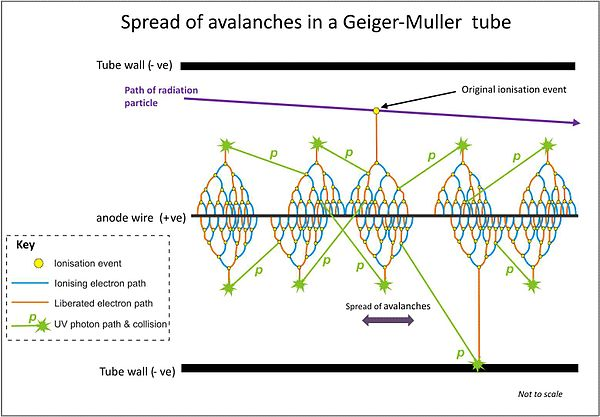
\includegraphics[scale=0.70]{pictures/Chap3/avalanche.jpg}
\caption{Picture explaining a Townsend avalanche, an incident particle interacts in the gas and ionize it. The created electron drifts to the cathodic wire due to the electric field and generates an avalanche. Some emitted photons can also ionize the gas and create another avalanche.}
\label{avalancheTownsend}
\end{center}
\end{figure}


\NI In most of the case, the wire chambers are filled with a noble gas because of their interesting characteristics. They are mono-atomic (no rotation or vibration), easy to purify and not electronegative. At the end of the discharge, during the recombinaison, an electron can be extracted from the cathode and re-create an avalanche. To avoid this phenomena, a small amount of a quenching gas is added.


\bigskip


\NI The great gain of the Geiger mode (between 10$^\text{6}$ and 10$^\text{8}$) allows to reach high sensitivity detection but unfortunately does not allowed to know the nature of the particle and their energy. Another drawback of the wire chambers working in Geiger mode is the long dead time (few hundred $\mu$s). This dead time is not an obstacle in NEMO detector since the rate is expected to be at the Hertz order.    




\begin{figure}[h!]
\begin{center}
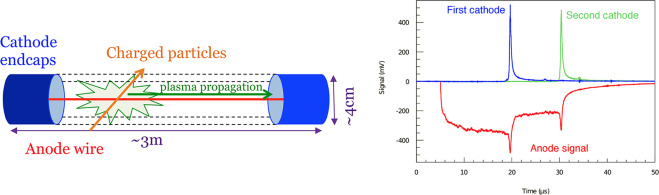
\includegraphics[scale=0.80]{pictures/Chap3/trackerSchema.jpg}
\caption{Left : Geiger cell of the tracker. The red line represents the anode wire surrended by 8 cathode wires attached to cathod endcaps (represented by the dashed lines). Right : anodic and cathodic signals detected.}
\label{trackerSignal}
\end{center}
\end{figure}



\subsubsection{Calorimeter}


\NI The calorimeter of NEMO experiments is composed of plastic scintillator blocks coupled with photomultiplier tubes (PMT). By interacting inside the block, a particle will excite the electrons of the medium which will de-excite by emitting visible light. This scintillation light is then collected by a PMT. The energy of the incident particle can be determine thanks to the amount of scintillation light. In case of plastic scintillator only a small fraction of the kinetical energy of the incident particle is converted in light. The majority of the energy leaves under a non radiative way (phonon, heat). The light yield per path length (dL/dx) can be estimated with the Birks' law : 


\begin{equation}
\frac{\text{dL}}{\text{dx}} = \frac{\text{S}~(\frac{\text{dE}}{\text{dx}})}{\text{1}+\text{k}_\text{B}~(\frac{\text{dE}}{\text{dx}})}
\end{equation}


\NI where S is the scintillation efficiency, dE/dx is the energy loss of the particle per path length and k$_\text{B}$ is the Birks' constant which depends on the scintillator material. 


\bigskip


\NI A part of the scintillation light can be re-absorbed by the block material. In order to avoid this phenomena another materials can be introduced inside the block to shift the wave length. This wave length shifter composent improve the transparency and also has the advantage of emitting light in the acceptance range of the PMT. 


\bigskip


\NI Coupled directly or indirectly (a light guide can be interposed) to the scintillation block, a PMT recovers the light to convert it into an electric signal. A PMT is made of a photocathode, dynodes and an anode placed in a vacuum tube. The photocathode converts the incident photons by photoelectric effect into low energetic electrons in a linear yield. At this stage, the number of photo-electrons is still too low to provide an electric signal. These photo-electrons are directed to the first dynode thanks to the focusing electrode where they will be multiplied. By putting dynodes one after the other and appliying an higher positive voltage than the previous one, the signal is highly amplify. The collected signal by the anode is proportionnal to the energy of the incident photon. Figure~\ref{PMT} presents a simplified view of a PMT.


\begin{figure}[h!]
\begin{center}
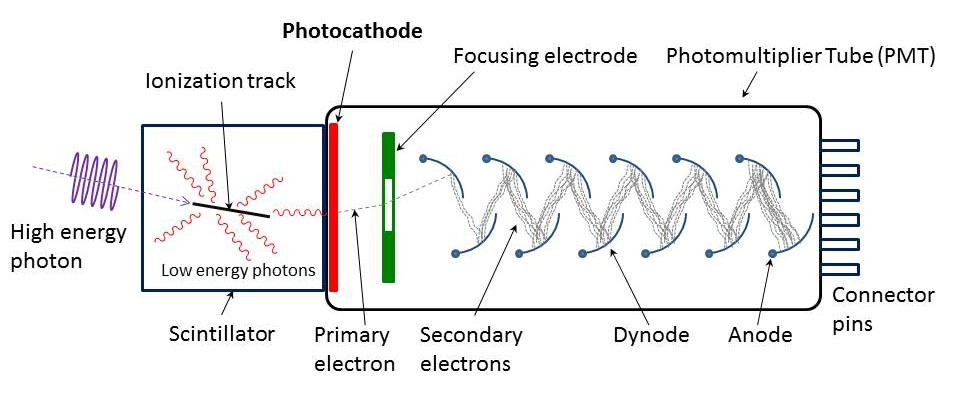
\includegraphics[scale=0.35]{pictures/Chap3/PhotoMultiplierTubeAndScintillator_v2.jpg}
\caption{Simplified view summarizing the operation of a photomultiplier.}
\label{PMT}
\end{center}
\end{figure}


\bigskip


\NI In general a PMT is sensitive in ultraviolet and near infrared and have a very short response time (tens of ns). A PMT can be characterized by its quantum efficiency, its collection efficiency and its multiplication factor. The quantum efficiency ($\epsilon_\text{q}$) is the probability for an incindent photon to produce a photo-electron. Today, $\epsilon_\text{q}$ rarely  exceeds 20-30 \% and depends of the photon wavelength. In the electron multiplication mechanism, some electrons may deviate from their favorable trajectories and not contribute to the multiplication. This effect can be parametrized by the collection efficiency ($\epsilon_\text{c}$) which depends on the geometry and composition of the dynodes. Finally, the multiplication factor ($\delta$) is defined for each dynode as the ratio of number of emitted electrons by the number of incindent electrons.


\bigskip


\NI In the case where PMT is used in a strong magnetic field, the electron trajectories are curved and steer them away from the dynoded. That is why the PMT are often shielded with soft iron or $\mu$-metal. 


\FloatBarrier


\subsection{Modane underground laboratory}\label{sec:LSM}


\NI The Modane underground laboratory (LSM : Laboratoire Souterrain de Modane in french) is located in the Frejus tunnel at the border between France and Italy (Figure~\ref{LSMtunnel}).  Sheltered from cosmic rays, the laboratory have been inaugurated in 1982 under 1700~meters of rocks (4200 meter water equivalent) which makes it the deepest underground laboratory in Europe and the third one in the world. The cosmic ray flux inside the laboratory have been estimated to be 4.m$^\text{-2}$.j$^{\text{-1}}$, compared to the million of particles arriving per m$^\text{2}$ at the surface of the Earth. Figure~\ref{LabDeepth} shows the total muon flux according the depth for different underground laboratory around the world. 


\bigskip


\begin{figure}[h!]
\begin{center}
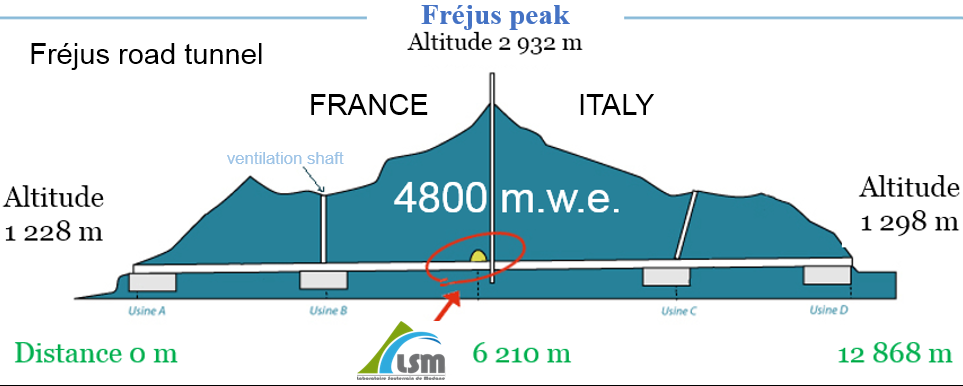
\includegraphics[scale=0.40]{pictures/Chap3/LSMtunnel.png}
\caption{Schematic view of the Modane underground laboratory location in the Frejus tunnel.}
\label{LSMtunnel}
\end{center}
\end{figure}


\NI The protected environment of the laboratory is very conducive to the searches requiring a very low background. Initially, the laboratory hosted an experiment searching for the proton decay. Latest, the laboratory diversified its activities, including astrophysics (mainly for the searches for the dark matter), biology, geology, electronics and environmental studies. The laboratory also have several High Purity Germanium detectors (HPGe) to measure very low radioactivity. 


\begin{figure}[h!]
\begin{center}
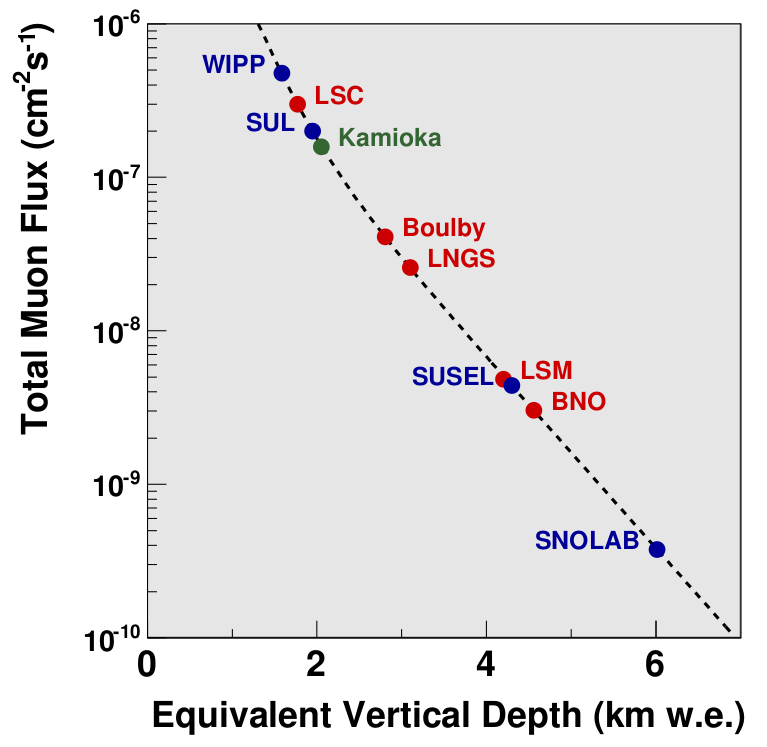
\includegraphics[scale=0.27]{pictures/Chap3/lab_depth.png}
\caption{Total muon flux in cm$^{\text{-2}}$.s$^{\text{-1}}$ with respect to the depth for different underground laboratory.}
\label{LabDeepth}
\end{center}
\end{figure}


\NI LSM hosted NEMO-2 detector at the end of the 80's. Then NEMO-3 have been installed and took data between 2003 and 2011. Today NEMO-3 have been replaced by SuperNEMO demonstrator which is currently under construction and commissionning phase.


\FloatBarrier


\subsection{NEMO-1 and NEMO-2}\label{sec:NEMO1-2}


\NI Before to build a large scale detector, the collaboration wanted to ensure validity of electron reconstruction at low energy with the tracking device. Two prototypes have been built, NEMO-1 and NEMO-2, which also allow to understand important points for improving the sensitivity of the future detectors. 

\subsubsection{NEMO-1}

\NI The first prototype NEMO-1 was built in 1988. In a first step, the detector took data with cosmic at the sea level and then  have been moved at LSM where it worked during 18 months. NEMO-1 demonstrated that the track reconstruction of the low energetic electrons is possible until few hundred keV. This prototype was also useful to study the shielding and to measure the radioactivity inside the wire chamber.


\bigskip


\NI The trajectory of the electron was reconstructed thanks to 64 Geiger cells made of a central wire surrounded by 8 ground wires of 1 meter long (8 $\times$ 8). The tracker volume was filled with gaseous helium and 2\% of ethanol as quencher. The final gas density was 0.2 mg.cm$^{\text{-2}}$ which limit the energy loss of the electron (loss of 14 keV for an electron of 1 MeV crossing 50~cm of the gas).


\bigskip


\NI The energy of the electrons was measured thanks to 2 plastic scintillators planes surrounding the tracker volume and measuring 0.28 $\times$ 0.02 $\times$ 1.0 m$^{\text{3}}$. Each plane was divided into 2 parts coupled with a PMT. 


\bigskip


\NI To be protected from the background, the detector was shielded with iron and lead for a total width of 20~cm lead equivalent.


\subsubsection{NEMO-2}


NEMO-2 is the second prototype built by the collaboration. Around 10 times bigger than NEMO-1, its main goal was the study of the background and the validation of the strategy to measure them via different channels. A schematic view of the detector is presented in Figure~\ref{NEMO2}.


\begin{figure}[h!]
\begin{center}
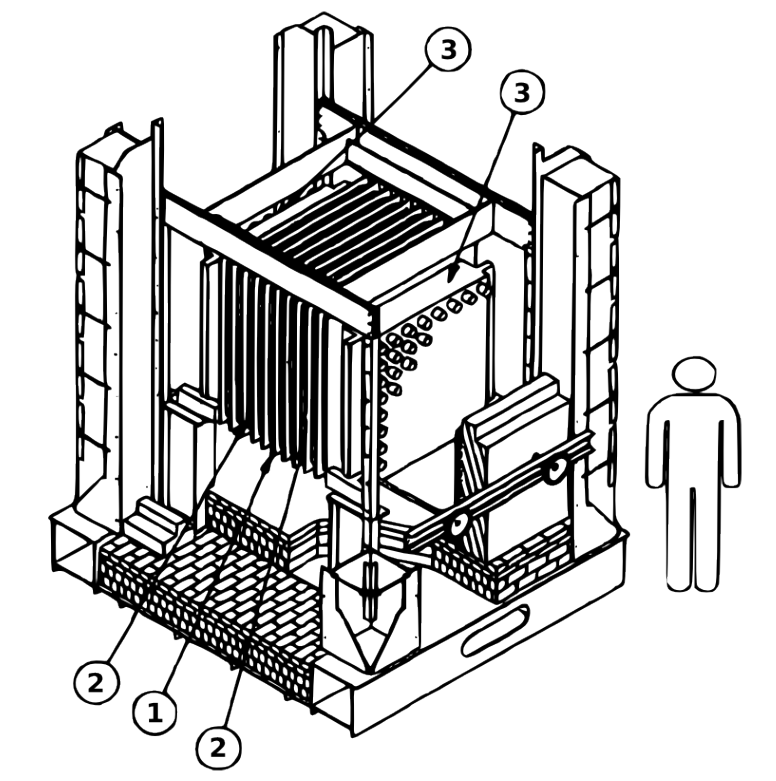
\includegraphics[scale=0.27]{pictures/Chap3/NEMO2.png}
\caption{Schematic view of the NEMO-2 detector. (1) central frame supporting the $\beta\beta$ source, (2) copper frame holding the Geiger cells, (3) 8 $\times$ 8 scintillators coupled to PMT.}
\label{NEMO2}
\end{center}
\end{figure}

\bigskip


\NI The source frame is the central part of the detector, labelled (1) in~Figure~\ref{NEMO2}. Measuring~1~m$^\text{2}$, this frame hold different $\beta\beta$ isotopes during several phases between 1991 and 1995. The results obtained for the double beta decay of these isotopes are summarized in Table~\ref{NEMO-2-results}.


\begin{table}[h!]
\centering
\begin{tabular}{c|c|c}
Isotope           & Mass (nat. + enr.) [g] &T$_{\text{1/2}}$ $\times$ 10$^{\text{19}}$ [y] at 90 \% C.L. \\[0.05cm]
\toprule
$^{\text{116}}$Cd & 143 + 152   & 3.75 $\pm$ 0.35 (stat.) $\pm$ 0.21 (syst.)  \cite{NEMO2:Cd116}\\[0.05cm]
$^{\text{100}}$Mo & 163 + 172   & 0.95 $\pm$ 0.04 (stat.) $\pm$ 0.09 (syst.)  \cite{NEMO2:Mo100}\\[0.05cm]
$^{\text{82}}$Se  & 134 + 157   & 8.30 $\pm$ 1.00 (stat.) $\pm$ 0.70 (syst.)  \cite{NEMO2:Se82}\\[0.05cm]
$^{\text{96}}$Zr  & 18.3 + 20.5 & 2.1 $^{+\text{0.8}}_{-\text{0.4}}$ (stat.) $\pm$ 0.2 (syst.) \cite{NEMO2:Zr96} \\[0.05cm]
\bottomrule
\end{tabular}
\caption{Results of the search for double decay with the NEMO-2 detector. The second column presents the isotope mass introduced (natural and enriched).}
\label{NEMO-2-results}
\end{table}  


\bigskip


\NI The source frame was surrounded on each side by 5 copper frames holding 640 Geiger cells (320 horizontal and 320 vertical), labelled (2) in~Figure~\ref{NEMO2}. The tracking volume was filled with gaseous helium and 4\% of ethanol for quenching. The transverse resolution was 500 $\mu$m and the longitudinal resolution was 4.7 mm. 


\bigskip


\NI The energy and the time of light of the electrons was obtained thanks to 2 planes of 8 $\times$ 8 plastic scintillators (for a total of 128 PMTs), labelled (3) in~Figure~\ref{NEMO2}. The distance between the source and the calorimeter was 50 cm. The dimensions of each scintillator block was 12~$\times$~12~cm$^{\text{2}}$ with a depth of 2~cm$^{\text{2}}$ to fully contain the electrons with an energy up to 4 MeV. Light guide was installed between scintillator and PMT. The calorimeter energy resolution (FWHM) was 18\% at 1 MeV with a time resolution of 275 ps (550 ps at 0.2 MeV). A laser and optical fiber was introduced close to PMTs to check the stability of the scintillation detectors. Finally, the tracking volume and scintillators were surrounded by a lead (5~cm) and iron (20~cm) shield.



\bigskip


\NI NEMO-2 demonstrated that the background coming from the radon was important and its reduction was crucial to scale the experiement up.   


\FloatBarrier


\section{NEMO-3}\label{sec:NEMO3}


\NI The NEMO-3 detector took data between January 2003 and January 2011 and search for $\beta\beta$ decays among 7 different isotopes.


\subsection{General design}

\NI NEMO-3 adopted a cylindrical geometry in order to optimise the volume of the detector with respect to the foils surface. The detector was divided into 20 identical sectors. A exploded view of the detector is shown in Figure~\ref{NEMO3Detector}.


\bigskip

\NI The sources were verticaly disposed forming a cylinder of 3.1 of diamater and 2.5 meters high for a total surface of around 20 m$^\text{2}$. Several isotopes in different proportion were placed in the detector. On each side of the source foil, a total of 6180 Geiger cells allow the track reconstruction in 3 dimensions. Plastic scintillators coupled with low radioactivity PMT surrounded the wire chamber. 


\bigskip


\NI A solenoid surrounding entirely the detector produced a 25~Gauss magnetic field parallel to the foil axis, in order to identify the particle charge. The detector was shielded from photons with 19~cm of iron, 30~cm of borated water on the sides parts and 28~cm of wood on the top and bottom sides thermalize fast neutrons and capture thermal neutrons.  


\begin{figure}[h!]
\begin{center}
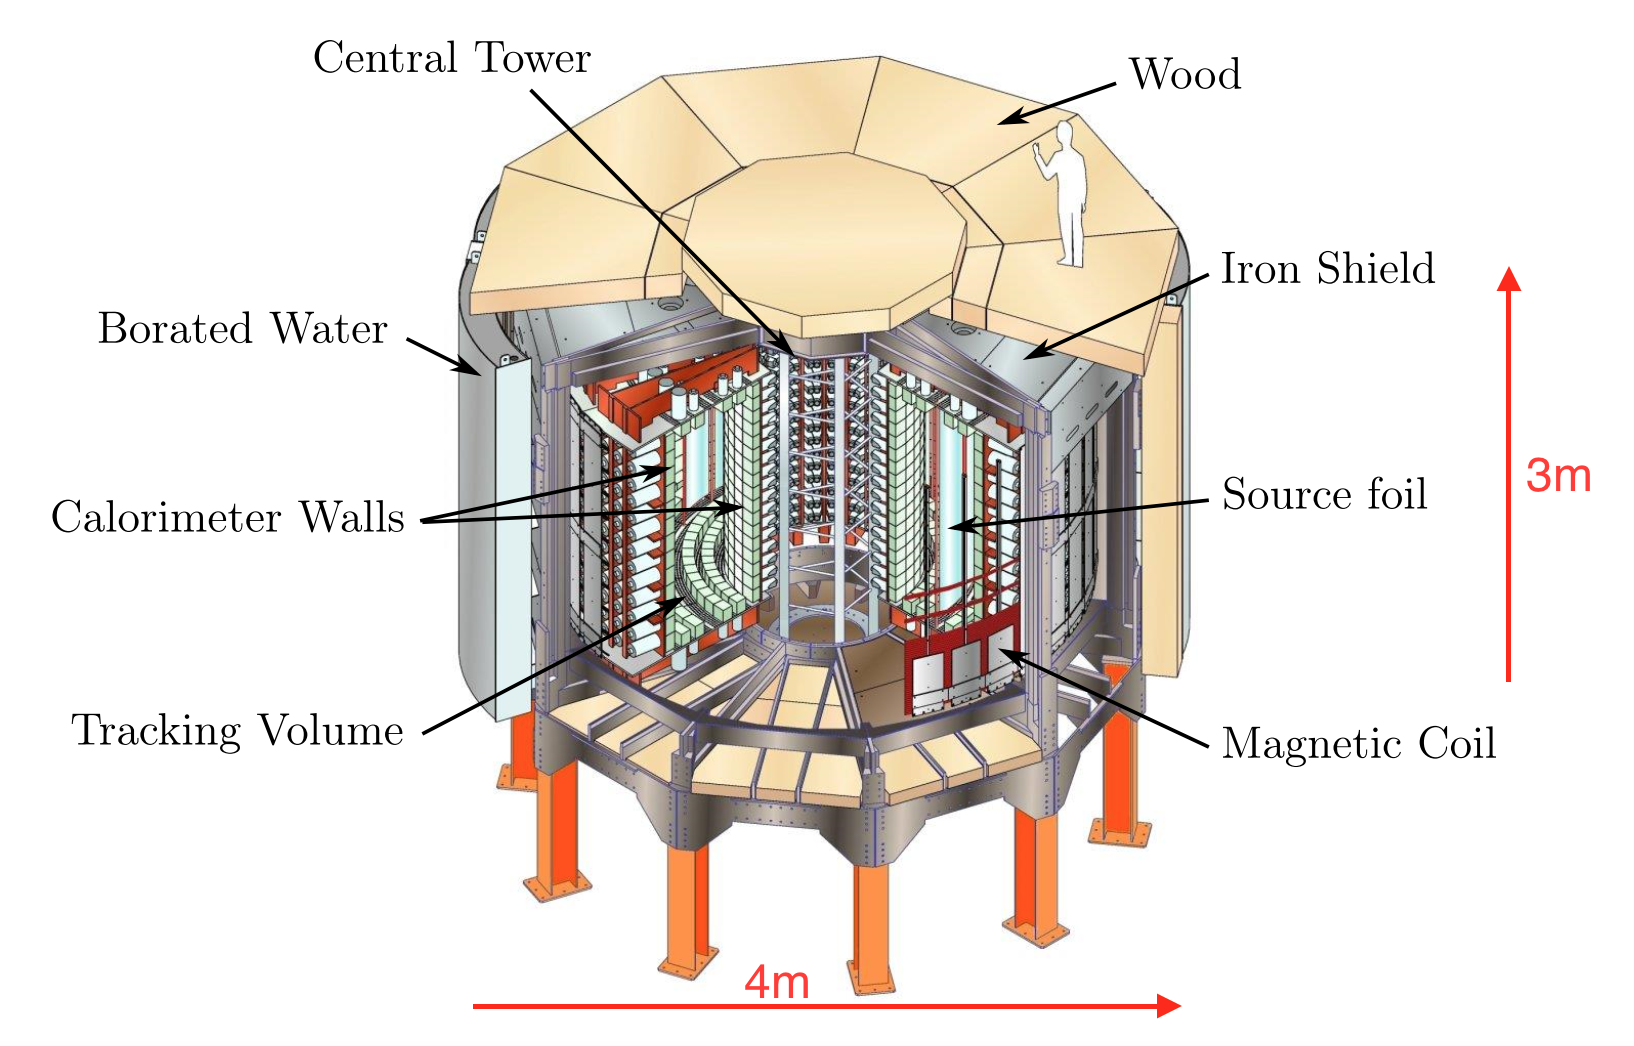
\includegraphics[scale=0.50]{pictures/Chap3/DetectorCrossSection.png}
\caption{Schematic view of the NEMO-3 detector.}
\label{NEMO3Detector}
\end{center}
\end{figure}


\begin{figure}[h!]
\begin{center}
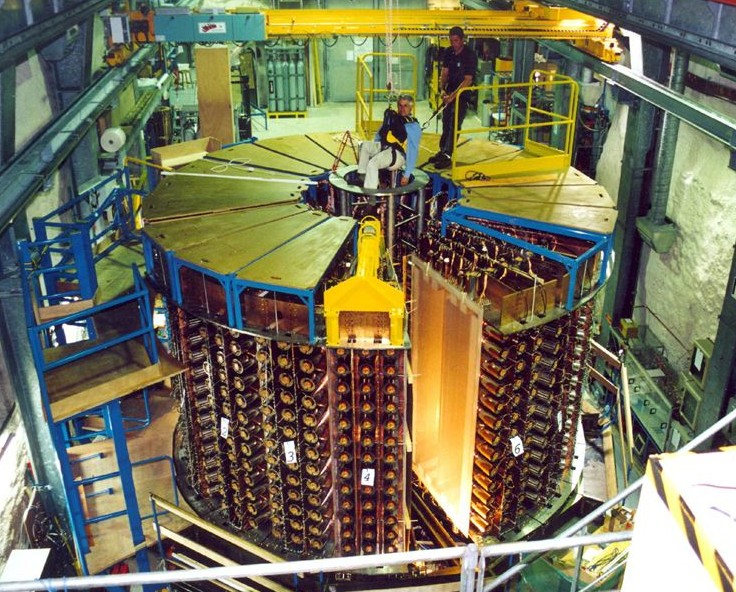
\includegraphics[scale=0.40]{pictures/Chap3/photoNEMO3.jpg}
\caption{Picture of the NEMO-3 detector in LSM before the installation of the last sector. The coil generating the magnetic field and the different shildings are not present.}
\label{NEMO3Photo}
\end{center}
\end{figure}


\FloatBarrier


\subsection{Source foils}

\NI The separation of the source foils from the rest of the detector give to NEMO-3 the great advantage to place different isotopes. This may allow to confirm a possible excess in the 0$\nu\beta\beta$ region with several atoms and test the results being less dependant of the nuclear matric element evaluations and by better controlling the backgrounds. The choice of which isotopes to study has mainly been determined by the following criteria (summarized in Table~\ref{tab:isotopeNEMO3} for the isotopes introduced in NEMO-3) : 


\begin{itemize}
\item the transition energy (Q$_{\beta\beta}$) : the higher this value is, the less the natural radioactivity is troublesome. The minimal value is 2.615~MeV which correspond to the higher $\gamma$-ray energy produced in natural radioactivity (decay of $^{\text{208}}$Tl).


\item the half-life of the 2$\nu\beta\beta$ process (T$_{\text{1/2}}^{\text{2}\nu}$) : the higher this value is, the less the number of 2$\nu\beta\beta$ events in the Q$_{\beta\beta}$ region is high.  


\item the natural isotopic abundance : in general the higher the abundance the easier the enrichment process. Only isotopic abundances greater than 2 \% were considered. 
\end{itemize}


\bigskip


\NI Five nuclei are quite satisfying : $^{\text{100}}$Mo, $^{\text{82}}$Se, $^{\text{116}}$Cd, $^{\text{96}}$Zr and $^{\text{150}}$Nd. The $^{\text{100}}$Mo (7~kg) and $^{\text{82}}$Se (0.9~kg) isotopes have been introduced for the search for 0$\nu\beta\beta$ decay. Smaller amount of $^{\text{116}}$Cd (405~g), $^{\text{150}}$Nd (37~g) and $^{\text{96}}$Zr (9.4~g) have also been inserted for 2$\nu\beta\beta$ decay studies. Even if $^{\text{48}}$Ca does not meet the criteria (very small natural abundance), $\sim$7~g have been introduced because of its impressive Q$_{\beta\beta}$ value which may allow a background free approach. 454~g of $^{\text{130}}$Te have also been added for 2$\nu\beta\beta$ studies (because of its high natural abundance). Foils made of copper (not a $\beta\beta$ emitter) and natural tellurium have been introduced in order to control the background measurements. The location of the sources among the different sectors are shown in Figure~\ref{NEMO3Sector}.


\bigskip



\begin{table}[h!]
\centering
\begin{tabular}{c|c|c|c|c}
Isotopes & Mass [g] & Q$_{\beta\beta}$ [MeV] & T$_{\text{1/2}}^{\text{2}\nu}$ [y] & Abundance [\%]\\[0.05cm]
\toprule
$^{\text{100}}$Mo & 6 914 & 3.034 & 7.2 $\times$ 10$^{\text{18}}$ & 9.63 \\[0.1cm]
$^{\text{82}}$Se  & 932   & 2.995 & 9.6 $\times$ 10$^{\text{19}}$ & 8.73 \\[0.1cm]
$^{\text{130}}$Te & 454   & 2.529 & 7.0 $\times$ 10$^{\text{20}}$ & 33.8 \\[0.1cm]
$^{\text{116}}$Cd & 405   & 2.802 & 2.9 $\times$ 10$^{\text{19}}$ & 7.49 \\[0.1cm]
$^{\text{150}}$Nd & 37    & 3.367 & 9.1 $\times$ 10$^{\text{18}}$ & 5.6  \\[0.1cm]
$^{\text{96}}$Zr  & 9.4   & 3.350 & 2.4 $\times$ 10$^{\text{19}}$ & 2.8  \\[0.1cm]
$^{\text{48}}$Ca  & 6.99  & 4.271 & 4.4 $\times$ 10$^{\text{19}}$ & 0.19 \\[0.1cm]
\bottomrule
\end{tabular}
\caption{Mass, Q$_{\beta\beta}$, T$_{\text{1/2}}^{\text{2}\nu}$ and abundance of the different isotopes introduced in NEMO-3.}
\label{tab:isotopeNEMO3}
\end{table} 




\begin{figure}[h!]
\begin{center}
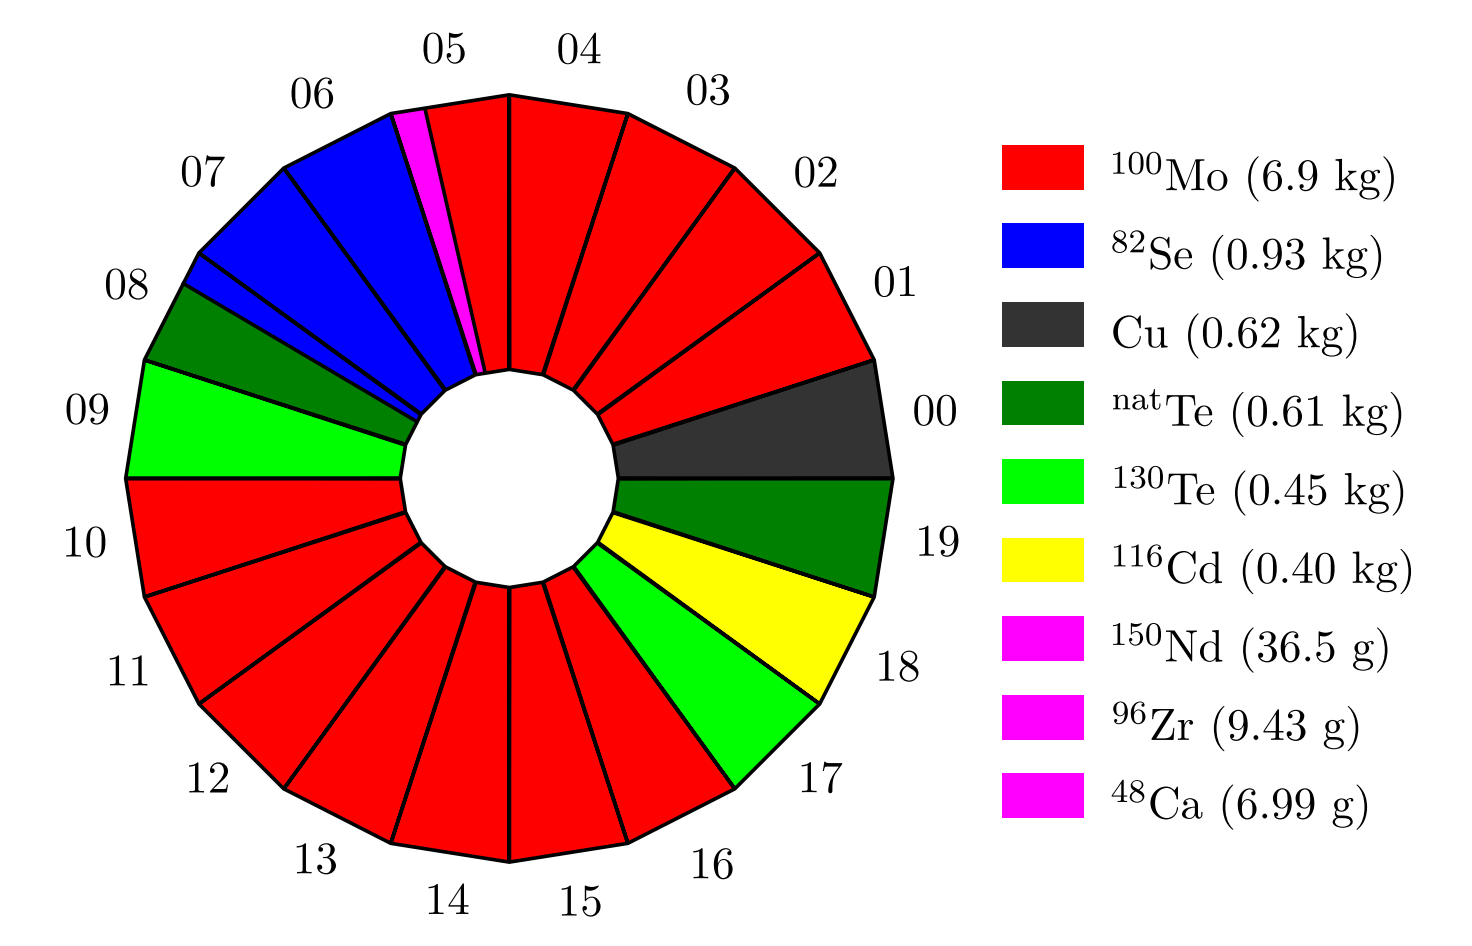
\includegraphics[scale=0.50]{pictures/Chap3/BBSourceDistribution.png}
\caption{Schematic view of the seven different $\beta\beta$ sources location inside the NEMO-3 detector. The main isotopes was $^{\text{100}}$Mo (6.9~kg) and $^{\text{82}}$Se (0.9~kg). Copper foils have been installed for background measurements.}
\label{NEMO3Sector}
\end{center}
\end{figure}


\FloatBarrier


\NI Each sector supports a source frame where 7 strips were placed. The mean length of the strips was 2.48~m. The width of the strips was 6.3~cm except for the 2 strips at the border (6.5~cm). The surface density of the source foils (equivalent to the thickness) had been determined from simulations. The detector efficiency for the 0$\nu\beta\beta$ process is not compromised
as long as the surface densities of the foils do not exceed 60 mg/cm$^\text{2}$ (limited by the energy resolution of the calorimeter). As consequence, the thickness of the metallic foils (cadmium, copper and a part of molybdenium) does not exceed 60~$\mu$m. The composite foils, which are a mixture of source powder and radiopure organic glue (selenium, tellurium, zirconium, neodynium and cadmium), does not exceed 300~$\mu$m. 


\bigskip


\NI All these $\beta\beta$ isotopes mainly provide from the Earth's crust (directly extracted or by-product of the extraction) and contain impurities ($^{\text{238}}$U and $^{\text{232}}$Th) which during their decay generate events similar to $\beta\beta$ events. To remove these impurities, the sample must be purify by physical or chemical technique. Some purification techniques are detailled in Appendix \ref{sec:PurificationMethods}.


\subsection{Tracking volume}


\NI The tracking volume is made of vertical layers of 6180 Geiger cells (for a total of 39820 wires). The diameter of the wires and the gas composition have been studied during a long time to optimize the resolution and the efficiency of the tracker. The number of wires shoud not be too large to improve the transparency and avoid multiple scattering effects. The composition of the gas must allow a good reconstruction efficiency, limit the energy loss and the aging of the cells. The gas is a mixture of 95 \% of helium, 4 \% of ethanol, 1 \% of argon and 0.1 \% of water. 


\bigskip


\NI In cross-sectional view, each cell has a octogonal geometry with a diameter of 3~cm. The central anode wire is surrounded by 8 ground wires (4 are in common with the adjecent cells to limit the number of wires). An extra ground wire have been added between the layers to avoid electrostatic cross talk. The wires are made of stainless steel, 2.7~m long and 50~$\mu$m in diameter, and are stung by two iron petals which form the top and the bottom of the detector. At each cell extremity, a  cathode ring (3~cm long and 2.3~cm in diameter) was placed, the anode wire runs through the center of this
ring while the ground wires are supported just outside. An elementary Geiger cell is shown in Figure~\ref{GeigerCellNEMO3}.


\begin{figure}[h!]
\begin{center}
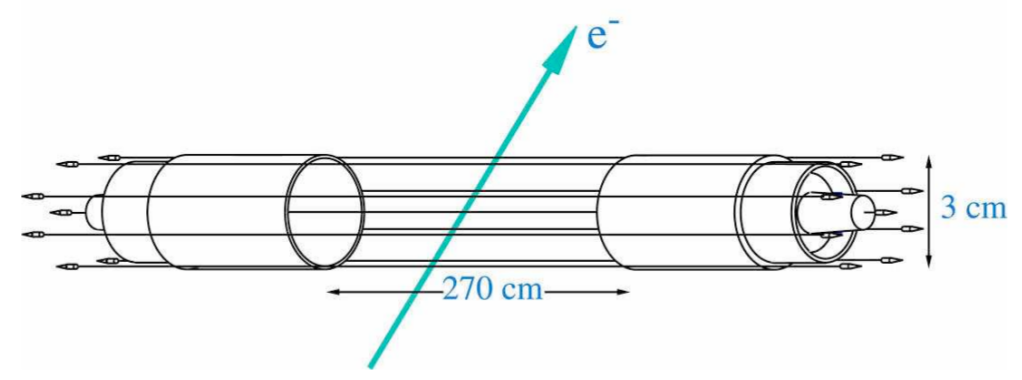
\includegraphics[scale=0.3]{pictures/Chap3/GeigerCellNEMO3.png}
\caption{Representation of an elementary Geiger cell in NEMO-3. The central anode wire of 270~cm length is surrounded by 8 ground wires. The cathod rings are shown at each end of the cell, 3~cm of diameter.}
\label{GeigerCellNEMO3}
\end{center}
\end{figure}


\NI The operating voltage for the anode wires was $\sim$1800~V. In this condition, a crossing charged particle creates around 6 electrons per centimiter. Close to the anode, these electrons drift towards the anode wire at a speed of about 2.3 cm/$\mu$s. Far away from the anode wire, the mean drift velocity is around 1 cm/$\mu$s. As explained before, the transverse position of the particle in the cells is reconstructed with the measurements of the drift times. The avalanche near the anode wire develops into a Geiger plasma which propagates along the wire at a speed of 6 to 7 cm/$\mu$s. The propagation times are used to determine the longitudinal position of the particle.


\bigskip


\NI The wire chamber was configured as 18 layers of Geiger cells parallel to the source foil, 4-2-3 layers on each side, as shown in Figure~\ref{TrackerNEMOView}. This configuration have been optimised by Monte-Carlo simulations. First, 4 layers are close to the source to precisely reconstruct the vertex location. The  tracker  allowed the reconstruction of the decay vertices on the foil with  an  average  resolution  of  0.5~mm  on  the  transversal plane (xy) and 8.0~mm on the longitudinal axis (z) for 1~MeV electron. Then 2 middle layers allow a good measurement of the track curvature. Finally, 3 layers close to scintillators are used to determine the impact point on the block in order to correct the energy measurement and improve the energy resolution of the electrons (the light collection is not uniform according the impact point).   




\begin{figure}[h!]
\begin{center}
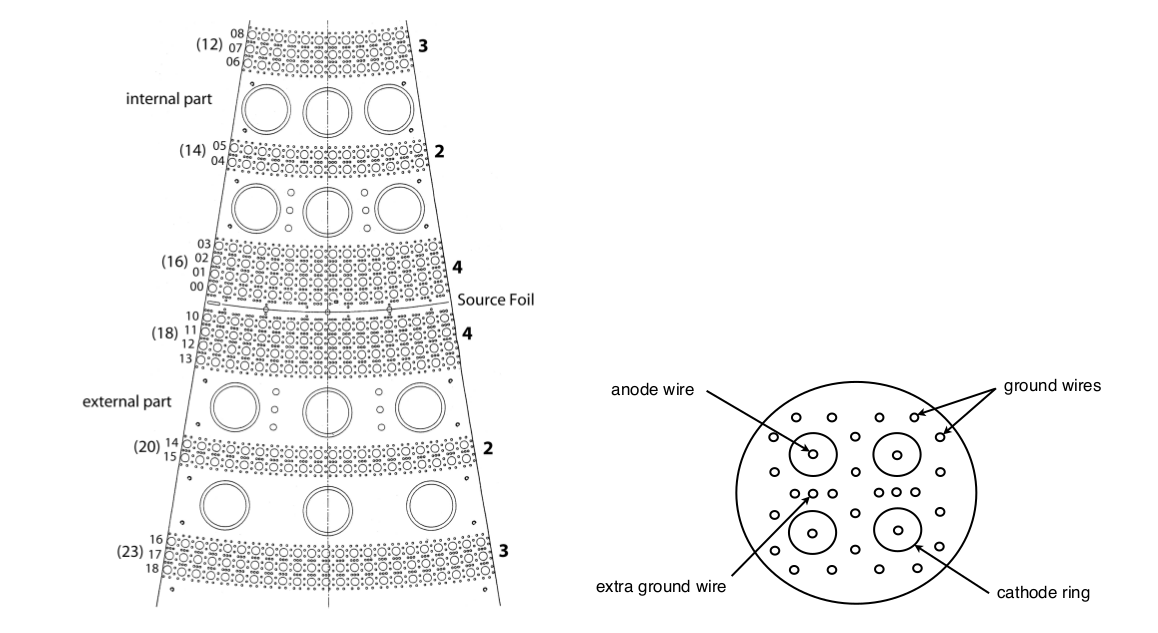
\includegraphics[scale=0.30]{pictures/Chap3/TrackerNEMOView.png}
\caption{Left : The 4-2-3 configuration of the Geiger cells in a NEMO-3 sector The 12 large rings represent the location of the light guides installed in the support structure to couple the scintillators to the PMTs. Right : Geiger
wiring of four elementary Geiger cells.}
\label{TrackerNEMOView}
\end{center}
\end{figure}


\bigskip

\NI The electronics of the wire chamber is split into two king of cards. The first one are dedicated to supply the high voltage of the anode (1620~V). The second cards constitutes the data acquisition. They are connected to the distribution cards. The first role of the acquisition is the amplification coming from the distribution cards. The computation of the cathodic and anodic time are realized. The anodic time corresponds to the difference between the trigger (given by the calorimeter) and the anodic signal, and is used to obtain the transversale position. The cathodic time corresponds to the difference between the arrival times of anodic and cathodic signals, useful to get the longitudinal position. The delayed signals are saved until 710 $\mu$s after the trigger in the aim of $^{\text{214}}$Bi measurements (Bipo cascades $^{\text{214}}$Bi whose the daughter nucleus $^{\text{214}}$Po have a helf-life of 164$\mu$s).  


\FloatBarrier


\subsection{Calorimeter}


\NI The NEMO-3 calorimeter is made of 1940 optical modules to measure the particle energy, make time of flight measurements and give a fast trigger signal. Each of optical module is made with a plastic scintillator, light guide and PMT (3'' or 5''). As shown in Figure~\ref{NEMO3Inside},  the scintillators blocks covered the inner and outer cylindrical walls of the detector, and also had limited coverage on the top and bottom (call petals). The gains of the PMTs have been adjusted to cover energies up to 12 MeV. The plastic scintillators have been chosen to minimize backscattering and for their radiopurity. The  calorimeter  provided  a  tim-ing  resolution  of $\sigma$ = 250~ps  while  the  energy  resolution  was $\sigma$E/E = 5.8~\%/$\sqrt{\text{E(MeV)}}$  for  the  scintillator coupled to 5'' PMTs, and 7.2~\%/$\sqrt{\text{E(MeV)}}$ for the scintillator equipped with 3" PMTs. 


\bigskip


\NI Two different kind of PMTs was used, the scintillator blocks of the internal walls and of the petals (except the petals close to the external wall) was coupled with R6091~3''~PMTs (1040 PMTs). These tubes are made of 12 dynodes and a flat photocathod. The blocks of the external wall and of the last petals were coupled to R6594~5''~PMTs (900 PMTs), having 10 dynodes and a hemispherical photocathode. A detailed schema of the location of the scintallator blocks in the NEMO-3 detector is presented in Figure~\ref{SectorDetailedPMTconfig}.


\smallskip


\begin{figure}[h!]
\begin{center}
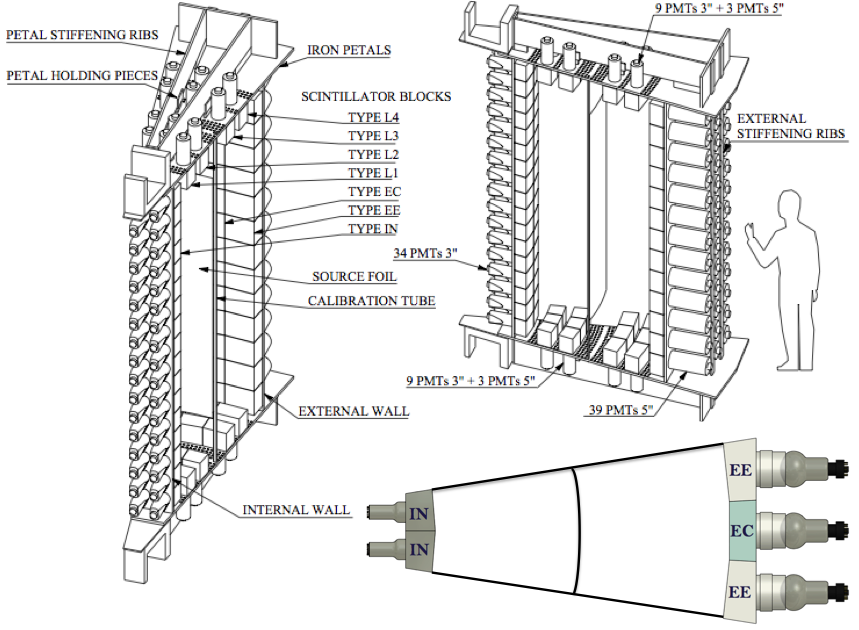
\includegraphics[scale=0.34]{pictures/Chap3/SectorDetailedPMTconfig.png}
\caption{One sector of NEMO 3 with details on the source foil, scintillator blocks and photomultipliers location.}
\label{SectorDetailedPMTconfig}
\end{center}
\end{figure}


\NI The scintillator was directly in contact with the gas of tracker. In order to prevent a rapid aging of the PMT due to the helium-alcohol gas, the blocks were supported by a rigid frame which allows the PMTs to be outside. To fit the cylindrical geometry of NEMO-3, 7 different types of scintillator have been specialy designed. 


\bigskip


\NI The block are mainly made of a styrene polymere (C$_\text{6}$H$_\text{5}$CH=CH$_\text{2}$), with a mean Z of 3.7 per atom), 2~cm of this material is able to contain a up to 3~MeV electron. On the other hand, the mean Z is too low to optimise the photon interaction. The thickness of all the blocks have been set to 10~cm to obtain an efficiency for $\gamma$-ray detection of 50~\% at 500~keV. The chemical nature of the scintillator is a solid solution of a scintillating agent p-Terphenyl (PTP). Some 1.4-di-(5-phenyl-2-oxazoly) benzene (POPOP) is added in polystyrene to shift the wavelength for a better detection by the PMT ($\lambda \approx$ 420~nm). After many years of study, the final composition of the scintillation block have been chosen to be : 98.49~\% of polystyrene, 1.5~\% of PTP, and 0.01~\% of POPOP for the blocks of the walls and 98.75 \% of polystyrene, 1.2~\% of PTP, and 0.05~\% of POPOP for the petals blocks.


\bigskip


\NI The radiopurity of the scintillator blocks have measured to be 430 and 60 times better than the low radioactivity PMT (respectively in $^{\text{214}}$Bi and $^{\text{208}}$Tl). The blocks were finally wrapped with aluminized Mylar to not lose the scintillation light. A 60~mm thick light guide made of PMMA is used for the scintillator and PMT interface and to protect PMTs from helium. The light transmission through the guides is 98~\% in the wavelength range 380-420~nm.


\bigskip


\NI Based on analysis on NEMO-2 data, the dominant external background comes from the PMT. The development and the use of low radioactivity background is then crucial. For NEMO-3, the requirements for the PMT glass radioactivity was lower than 1.7~Bq/kg in $^{\text{40}}$K, lower than 0.83~Bq/kg in $^{\text{214}}$Bi and lower than 0.17~Bq/kg in $^{\text{208}}$Tl. The Hamamatsu company was chosen to produce the PMTs, with the radiopurity of their glass being 100 to 1000 times better than standard glass. Furthermore, the performances of their PMTs have been tested and meet the specifications : an energy resolution of 4~\% at 1~MeV, a time resolution of 250~ns at 1~MeV, a good linearity up to 4~MeV and a low dark current.  


\begin{figure}[h!]
\begin{center}
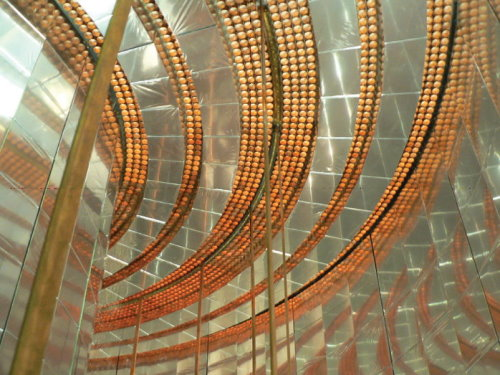
\includegraphics[scale=0.75]{pictures/Chap3/NEMO3Inside.jpg}
\caption{Inside view og the NEMO-3 wire chamber during disassembly. The reflective surfaces are the calorimeter walls and the copper parts support the Geiger cell wires.}
\label{NEMO3Inside}
\end{center}
\end{figure}



\NI Since the wires providing the high voltage of the PMTs are located inside the detector, they have to be made in radiopure materials. The PMT bases have been arranged with a progressive voltage divider in order to improve the linearity under high voltage conditions. All the PMT bases are supplied with 350~$\mu$A, the mean value of the high voltage is 1350~V for the 5'' PMT and 1800~V for the 3'' PMT. The length of the high voltage cables is the same 11~m with a positive tension (ground to the photocathode). In order to correct the different transit time (3 ns) between the two kind of PMT, the cable length are different for the output signals (11.3~m long for the 5'' PMT and 10.6~m long for the 3'' PMT). The 3 roles of the calorimeter are to measure the energy from the signal charge (ADC), measure the arrival time of the particles (TDC) and provide a quick trigger.


\FloatBarrier


\subsection{Magnetic coil and shielding}


\NI In order to reach the desired sensitivity for the effective neutrino mass, no events of external background have to be seen in the energy range [2.8 - 3.2]~MeV during 5 years of data taking. The external background is induced by the interactions of neutrons and photons with the detector or with the rocks surrounded the laboratory. It will be more described in Section~\ref{sec:externalBkg}. 


\bigskip


\NI Simulations based on NEMO-3 geometry and studies from NEMO-2 shown that the photon interaction with the source foil mainly generate a pair creation (e$^+$e$^-$) [ref : C. Marquet et al., NEMO collaboration, Nucl. Instr. and Meth. A457(2001) 487]. The installation of a solenoid capable of producing a 25~G magnetic field surrounded by external shields highly reduce the external background. The magnetic coil allows positron/electron discrimation during the shields stop the majority of photons and neutrons.  


\subsubsection{The magnetic coil}


\NI The magnetic field have been optimized to maintain a good electron detection efficiency and distinguish the charge of the particles. In case where the magnetic field is too intense, the electrons are too curved and can not reach the calorimeter. On the other hand, the field must be sufficient to curve the trajectory for a good charge discrimation. An chosen value of 25~G provides a rejection of 95~\% of the (e$^+$e$^-$) pair event.


\bigskip


\NI The cylindrical coil surronds entirely the detector is made of 10 sections with 203 copper rings connecting every other sector to form one loop of the helix as shown in Section~\ref{NEMO3Detector}. The coil is 5320 mm in diameter, 2713 mm in height and has a mass of 5 tons ($\sim$ 3.1 tons of high radiopurity copper). To generate 25~G the required current is 29~A, and by taking account the resistivity of the copper rings (1.6 $\times$ 10$^{\text{-8}}$~$\Omega$), the total resistance of the coil is 0.6~$\Omega$. Fans have been placed in each section of the iron shield (Flow rate 1~m$^\text{3}$/s) are sufficient to cool the coil and the PMTs.



\subsubsection{The shieldings}


\NI To restrain the troublesome flux of photons and neutrons two shields have been installed. The first one is made of 20~cm (18~cm at few places to fit with the mechanical support) of radiopure iron spit into ten sections (165 tons) with two end-caps (6 tons each). This first shield reduces the $\gamma$-ray and thermal neutron fluxes. The second one have been optimized to suppress the contribution of slow and fast neutrons (up to few MeV). It is made itself of 3 parts :  20~cm of paraffin located below the central tower of the detector (not shown in Figure~\ref{NEMO3Detector}), 28~cm of wood placed below and above the detector, and 35~cm of borated water contained in tank covered the walls of the detector.  


\subsubsection{The anti-radon facility}


\NI As had been identified with the NEMO-2 detector, radon is troublesome and constitutes an important part of the background. During its decay chain, cascades of photons and electrons are emitted and can by different processes mimic the $\beta\beta$ signal. Despite all precautions taken to isolate the detector from the laboratory air with radon-tight seals, an excess of radon has been observed.  


\bigskip


\NI To fix this problem, a anti-radon facility have been installed at the end of 2004 made of an hermetic tent surrounding the entire detector flushed with radon-free air. Thanks to this system the radon concentration in the air around the detector is about 100 times lower than the air of the laboratory. The effect on the radon activity inside the tracker in shown in~Figure~\ref{RadonByTime}, a reduction of a factor $\sim$~7 has been measured.


\bigskip


\NI To purify the air from radon a trapping sytem using active coil (1 ton) have been deployed. The crossing of radon atoms is slow down. In case the crossing time is higher than the life time of radon the outcoming air is impoverished in radon. In order to increase the crossing time the trap is cold down at -50$^\circ$C. Using this device and by flushing (150 m$^\text{3}$/h) the outcoming air activity is around 10~mBq/m$^\text{3}$ in radon (compared to the 15~Bq/m$^\text{3}$ incoming).

 
\begin{figure}[h!]
\begin{center}
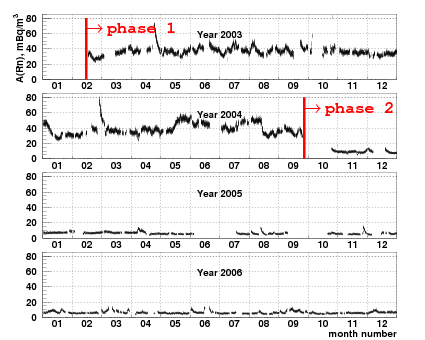
\includegraphics[scale=0.7]{pictures/Chap3/rn_bytime.png}
\caption{Radon activity measured inside the tracker. The level of radon is reduced by a factor $\sim$~7. The time periods preceding and following the anti-radon facility are respectively referenced as Phase 1 and Phase 2.}
\label{RadonByTime}
\end{center}
\end{figure}


\FloatBarrier


\subsection{Calibration system}

\NI To distinguish true 0$\nu\beta\beta$ events from various background processes (2$\nu\beta\beta$ decay is only experimentaly differentiable from 0$\nu\beta\beta$ by energy), a good calorimeter energy resolution is important. Thus a robust calibration procedure is needed to ensure and monitor the response of the calorimeter and detect any changes over the lifetime of the experiment. The NEMO-3 solution is the use of radioactive sources introduced inside the detector during runs dedicated to calibration. The absolute energy scale is determined during these runs (approximately one day every month), but the rest of the time, a laser survey system control the stability of the optical modules. 


\bigskip


\NI To introduce different calibration sources into the detector each sectors was equiped with a vertical tube made of flattened copper located along the edge of the source foils. The sources were placed along a narrow delrin rod (3 per rod at z~=~-90, 0 and +90~cm), and introduced by the top of the detector (after the removal of some shields). The position of the sources have been chosen to obain an uniform illumination of the scintillator blocks. This system allow to place the calibration sources close the $\beta\beta$ foils, thus the electron trajectories are very similar to the expected tracks in $\beta\beta$ events.


\bigskip


\NI Some studies shown that the response of the calorimeter was not the same for electrons and photons due to a difference in light collection. The electrons directly interact at the entrance of the scintillator while the photons interact deeper in the block. As we are interested by the electrons, the choice was made to use $^{\text{207}}$Bi and $^{\text{90}}$Sr sources. Decay of $^{\text{207}}$Bi provides conversion electrons of 482 and 976 keV. In order to not saturate the detector, the activity of the 60 sources of $^{\text{207}}$Bi should not be too high, each source have an activity around 6~nCi (222~Bq). To have access energies up to 3~MeV or more, an additional calibration point is got using electrons from $^{\text{90}}$Y (daughter of $^{\text{90}}$Sr) and the end-point of the $\beta$ spectrum at 2.283~MeV.


\bigskip


\NI For timing calibration of the detector, sources of $^{\text{60}}$Co are employed. These sources emits two $\gamma$-ray in  coincidence with energies of 1332 and 1173 keV. With the dispersion of arrival times differences, the delays between the 1940 channels is established. The activity of these sources can be high since the tracker is not required for this calibration.


\bigskip


\NI To monitor the stability of the calorimeter between absolute calibration runs, a calibration system of laser have been developed. Its main objective is to daily check the absolute energy and time calibrations. The PMTs linearity between 0 and 12~MeV is also determined also as the time-energy relation. In order to accomplish all these measurements, the shape of the laser signal must be very similar to the one produced by an electron and the emitted light has to be known with a high accuracy (< 1~\%) and stay stable. 


\bigskip


\NI The lasers used was di-azote lasers (N$_\text{2}$) with a wavelength of 337~$\pm$~15~nm. The light beam was divided into two parts. The first is directly sent to a photocathode to monitor the laser light intensity. To mimic the electron signal, the second beam is shifted to 420~nm with two optical filters. The light is then sent to the calorimeter blocks via optical fibers. Six independant reference blocks were equipped with $^{\text{207}}$Bi sources allowing to monitor the laser intensity by measuring energies of both the laser and the 976 keV conversion electrons.


\bigskip


\NI The relation between the charge signal and the energy deposited in the block is linear up to 4~MeV, which matches to the $\beta\beta$ region (the higher Q$_{\beta\beta}$ is 4.27~MeV for $^{\text{48}}$Ca) : 


\begin{equation}
\text{E} = \text{a} \times \text{(C - P) + b} 
\end{equation}


\NI where E is the energy, C the ADC value of the scintillator and P the pedestral. The energy calibration contants a and b are determined with at least two points from calibration sources measurements. In the simulation, the energy resolution is parametrized as :


\begin{equation}
\text{FWHM}^\text{2} \text{(E)} = \text{d} \times \text{E} + \text{e}
\end{equation} 

\NI where d $\times$ E coming from statistical fluctutations of the number of photoelectron arriving at the anode and of the number of scintillation photons. The parameter e represents the instrumental aspects independant of the energy.


\bigskip


\NI During the calibration phase using laser system, the last run is used to provide a reference energy for each optical module. In case the corrected gain (obtained with the laser system) is different from the gain get from $^{\text{207}}$Bi calibration sources a correction factor is applied.


\bigskip


\NI The cable length differences, the different geometry of the guide light and scintillator blocks or different PMT transit time can be responsible of different temporal response for two particle emitted in coincidence. In order to correctly calculate the time of flight of the particles and synchronize all the optical modules calibration sources of $^{\text{60}}$Co are used (2 $\gamma$-rays emitted in coincidence at 1332 et 1173 keV). Several runs of calibration changing the location of the sources have been taken.


\bigskip    


\NI Finally, thanks to the laser system, the time-energy dependance can be modeling by :


\begin{equation}
\text{t (C)} = \text{p}_\text{1} - \frac{\text{p}_\text{2}}{\text{p}_\text{3} \sqrt{\text{C}} + \text{p}_4}
\end{equation} 


\NI where C is the ADC value, all the other parameters ($p_i$) can be determined with the laser system in range [0-12]~MeV.


\FloatBarrier

\subsection{Results and measurements}


\NI After 5.25 years of data taking, NEMO-3 have been stopped and disassembled. The results on the searches for 2$\nu\beta\beta$ and 0$\nu\beta\beta$ are gathered in Table~\ref{tab:SummaryDecayRateNEMO3}. Most of these decay have been measured only by NEMO-3 or constitute the world best limits. The studies of the decays via the excited states and 0$\nu$4$\beta$ is also possible with the NEMO-3 detector.


\NI \textcolor{red}{ajouter les recherches concernant les états excités.}

\begin{table}[h!]
\centering
\begin{tabular}{c|c|c|c}
Isotopes & T$_{\text{1/2}}^{\text{2}\nu}$ [y] at 90 \% C.L. & T$_{\text{1/2}}^{\text{0}\nu}$ [y] at 90 \% C.L. & m$_{\beta\beta}$ [eV] \\
\toprule
$^{\text{100}}$Mo \cite{NEMO3:Mo100} & [7.1 $\pm$ 0.5] $\times$ 10$^{\text{18}}$ & > 1.1 $\times$ 10$^{\text{24}}$ & < [0.33 - 0.62]  \\[0.1cm]
$^{\text{82}}$Se \cite{NEMO3:Se82} & [10.07 $\pm$ 0.14 $\pm$ 0.54] $\times$ 10$^{\text{19}}$ & > 2.5 $\times$ 10$^{\text{23}}$  & < [1.2 - 3.0]  \\[0.1cm]
$^{\text{130}}$Te \cite{NEMO3:Te130}& [7.0 $\pm$ 0.9 $\pm$ 1.1] $\times$ 10$^{\text{20}}$ & > 1.3 $\times$ 10$^{\text{23}}$  & - \\[0.1cm]
$^{\text{116}}$Cd \cite{Arnold2016bed}& [2.74 $\pm$ 0.04 $\pm$ 0.18] $\times$ 10$^{\text{19}}$ & > 1.0 $\times$ 10$^{\text{23}}$  & < [1.4 - 2.5]  \\[0.1cm]
$^{\text{150}}$Nd \cite{NEMO3:Nd150}& [9.34 $\pm$ 0.22 $\pm$ $^{+\text{0.62}}_{-\text{0.60}}$] $\times$ 10$^{\text{18}}$ & > 2.0 $\times$ 10$^{\text{22}}$  & [1.6 - 5.3] \\[0.1cm]
$^{\text{96}}$Zr  \cite{NEMO3:Zr96}& [2.35 $\pm$ 0.14 $\pm$ 0.16] $\times$ 10$^{\text{19}}$ & 9.2 $\times$ 10$^{\text{21}}$  & - \\[0.1cm]
$^{\text{48}}$Ca \cite{NEMO3:Ca48} & [6.4 $\times$ $^{+\text{0.7}}_{-\text{0.6}}$ $^{+\text{1.2}}_{-\text{0.9}}$] $\times$ 10$^{\text{19}}$ & 2.0 $\times$ 10$^{\text{22}}$  & < [6.0 - 26] \\[0.1cm]
\bottomrule
\end{tabular}
\caption{Summary of the different half-lives measured for isotopes introduced in NEMO-3.}
\label{tab:SummaryDecayRateNEMO3}
\end{table}


\FloatBarrier


\section{SuperNEMO}\label{sec:SuperNEMO}


\NI Based on the NEMO-3 experiment, SuperNEMO is a new detector among the next generation searching for 0$\nu\beta\beta$. The strategy consists to take advantage of the previous detectors and increase the isotope mass of an improve the radiopurity. A total of 100~kg of isotopes could be studied allowing to reach 10$^{\text{26}}$~years on the 0$\nu\beta\beta$ process. The SuperNEMO project is composed of 20 identical modules. Thanks of several years of R\&D, great improvement have also been made concerning the energy resolution of the calorimeter. Table~\ref{tab:DifferenceNEMO3-SuperNEMO} summarizes the difference in performance for NEMO-3 detector and SuperNEMO project.


\begin{table}[h!]
\centering
\begin{tabular}{c|c|c}
      & NEMO-3 & SuperNEMO \\
\toprule
Mass~[kg] (main isotopes)           & 7 ($^{\text{100}}$Mo)         & 100 ($^{\text{82}}$Se)        \\[0.1cm]
 T$_{\text{1/2}}^{\text{2}\nu}$ [y] & 7.2 $\times$ 10$^{\text{18}}$ & 9.9 $\times$ 10$^{\text{19}}$ \\[0.1cm]
\midrule
Energy resolution & & \\
FWHM at 1~MeV                       & 15~\%                         & 8~\%                          \\[0.1cm]
FWHM at 3~MeV                       & 8~\%                          & 4~\%                          \\[0.1cm]
\midrule
Source radiopurity & & \\
A($^{\text{208}}$Tl)               & $\sim$ 100 $\mu$Bq/kg         & $<$ 2 $\mu$Bq/kg               \\[0.1cm]
A($^{\text{214}}$Bi)               & < 300 $\mu$Bq/kg              & < 10 $\mu$Bq/kg                \\[0.1cm]
\midrule
Level of radon A($^{\text{222}}$Rn)& $\sim$ 5.0 mBq/m$^\text{3}$ y   & < 0.1 mBq/m$^\text{3}$ y     \\[0.1cm]
\midrule
Sensitivity after 5~y of data taking & T$_{\text{1/2}}^{\text{0}\nu}$ > 10$^{\text{24}}$ & T$_{\text{1/2}}^{\text{0}\nu}$ > 10$^{\text{26}}$     \\[0.1cm]
\bottomrule
\end{tabular}
\caption{Summary of the difference in performance for NEMO-3 detector and SuperNEMO project.}
\label{tab:DifferenceNEMO3-SuperNEMO}
\end{table}  

\FloatBarrier


\subsection{The SuperNEMO demonstrator module}


\NI Before to build the 20 modules and in order to verify and validate the low level of background at large scale, the collaboration is building a first module called demonstrator module. This module will also serve to validate the technological choices (detection efficiency of the tracker, energy resolution of the calorimeter and source foil purification process). This module will contain 7~kg of $^{\text{82}}$Se in the form of thin source foils for physics study ($\sim$ 6.0 $\times$ 10$^{\text{24}}$~years on the 0$\nu\beta\beta$ process). 


\begin{figure}[h!]
\begin{center}
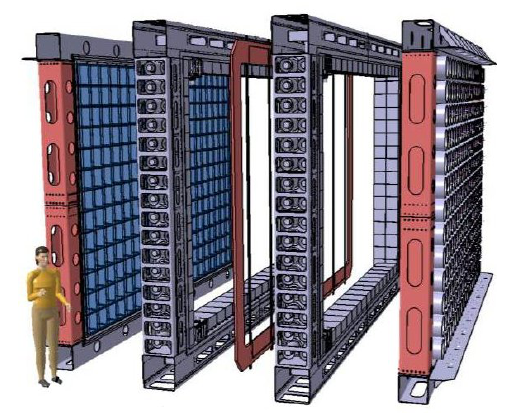
\includegraphics[scale=0.55]{pictures/Chap3/snemomodule.png}
\caption{Exploded view of one module of SuperNEMO. Thin source foils of $^{\text{82}}$Se are place at the center of the detector. 2 trackers modules made of 2034 Geiger cells reconstruct the electron tracks. 2 calorimeters walls measure the electron energies.}
\label{SuperNEMOexplodedView}
\end{center}
\end{figure}


\NI Figure~\ref{SuperNEMOexplodedView} presents a exploded view the demonstrator module. A planar geometry have been chosen. A central frame supports the thin foils of $\beta\beta$ emitters. The foils are sandwiched surrounded by the 2 tracker modules and 2 calorimeter walls inside water and iron shieldings. 


\FloatBarrier


\subsection{$^{\text{82}}$Se source foils}


\NI To choose the isotope of the demonstrator module a compromise must be find between many parameters. The choice have been made to use $^{\text{82}}$Se because of  its long 2$\nu\beta\beta$ half-life (to limit the irreducible background from 2$\nu\beta\beta$ in the search for 0$\nu\beta\beta$), its great Q$_{\beta\beta}$ (to limit the background coming from natural radioactivity) and a possible enrichment on a large scale. Some studies have been made for a possible used of $^{\text{150}}$Nd and $^{\text{48}}$Ca in a second phase of SuperNEMO.


\bigskip


\NI The source is divided in 36 foils (34 with 13.55 cm width and 2 with 12.5 cm width). A drawing of the source foil geometry can be found in Figure~\ref{SuperNEMOFoils}. The width of the total source is 485.7 cm, its height is 270.0 cm for a total surface of 131 139 cm$^\text{2}$ and a mean density of 55 mg/cm$^\text{2}$.


\begin{figure}[h!]
\begin{center}
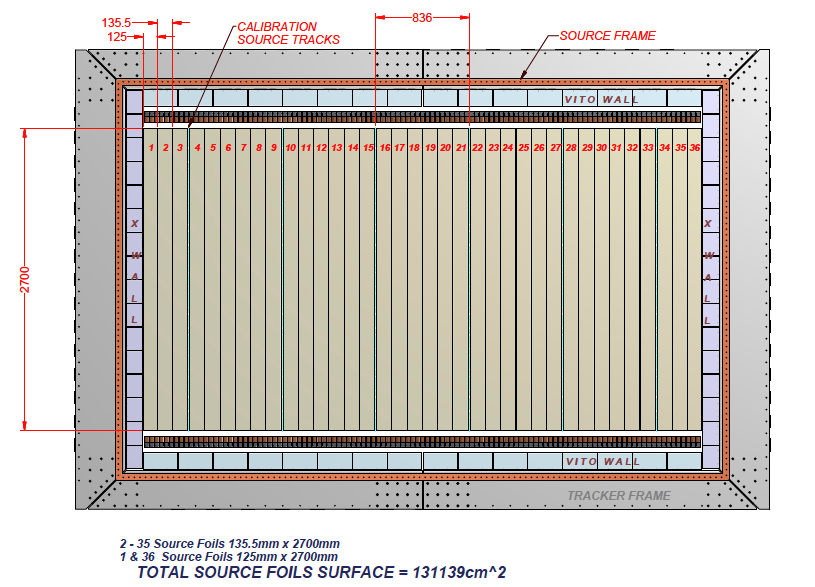
\includegraphics[scale=0.33]{pictures/Chap3/foil.png}
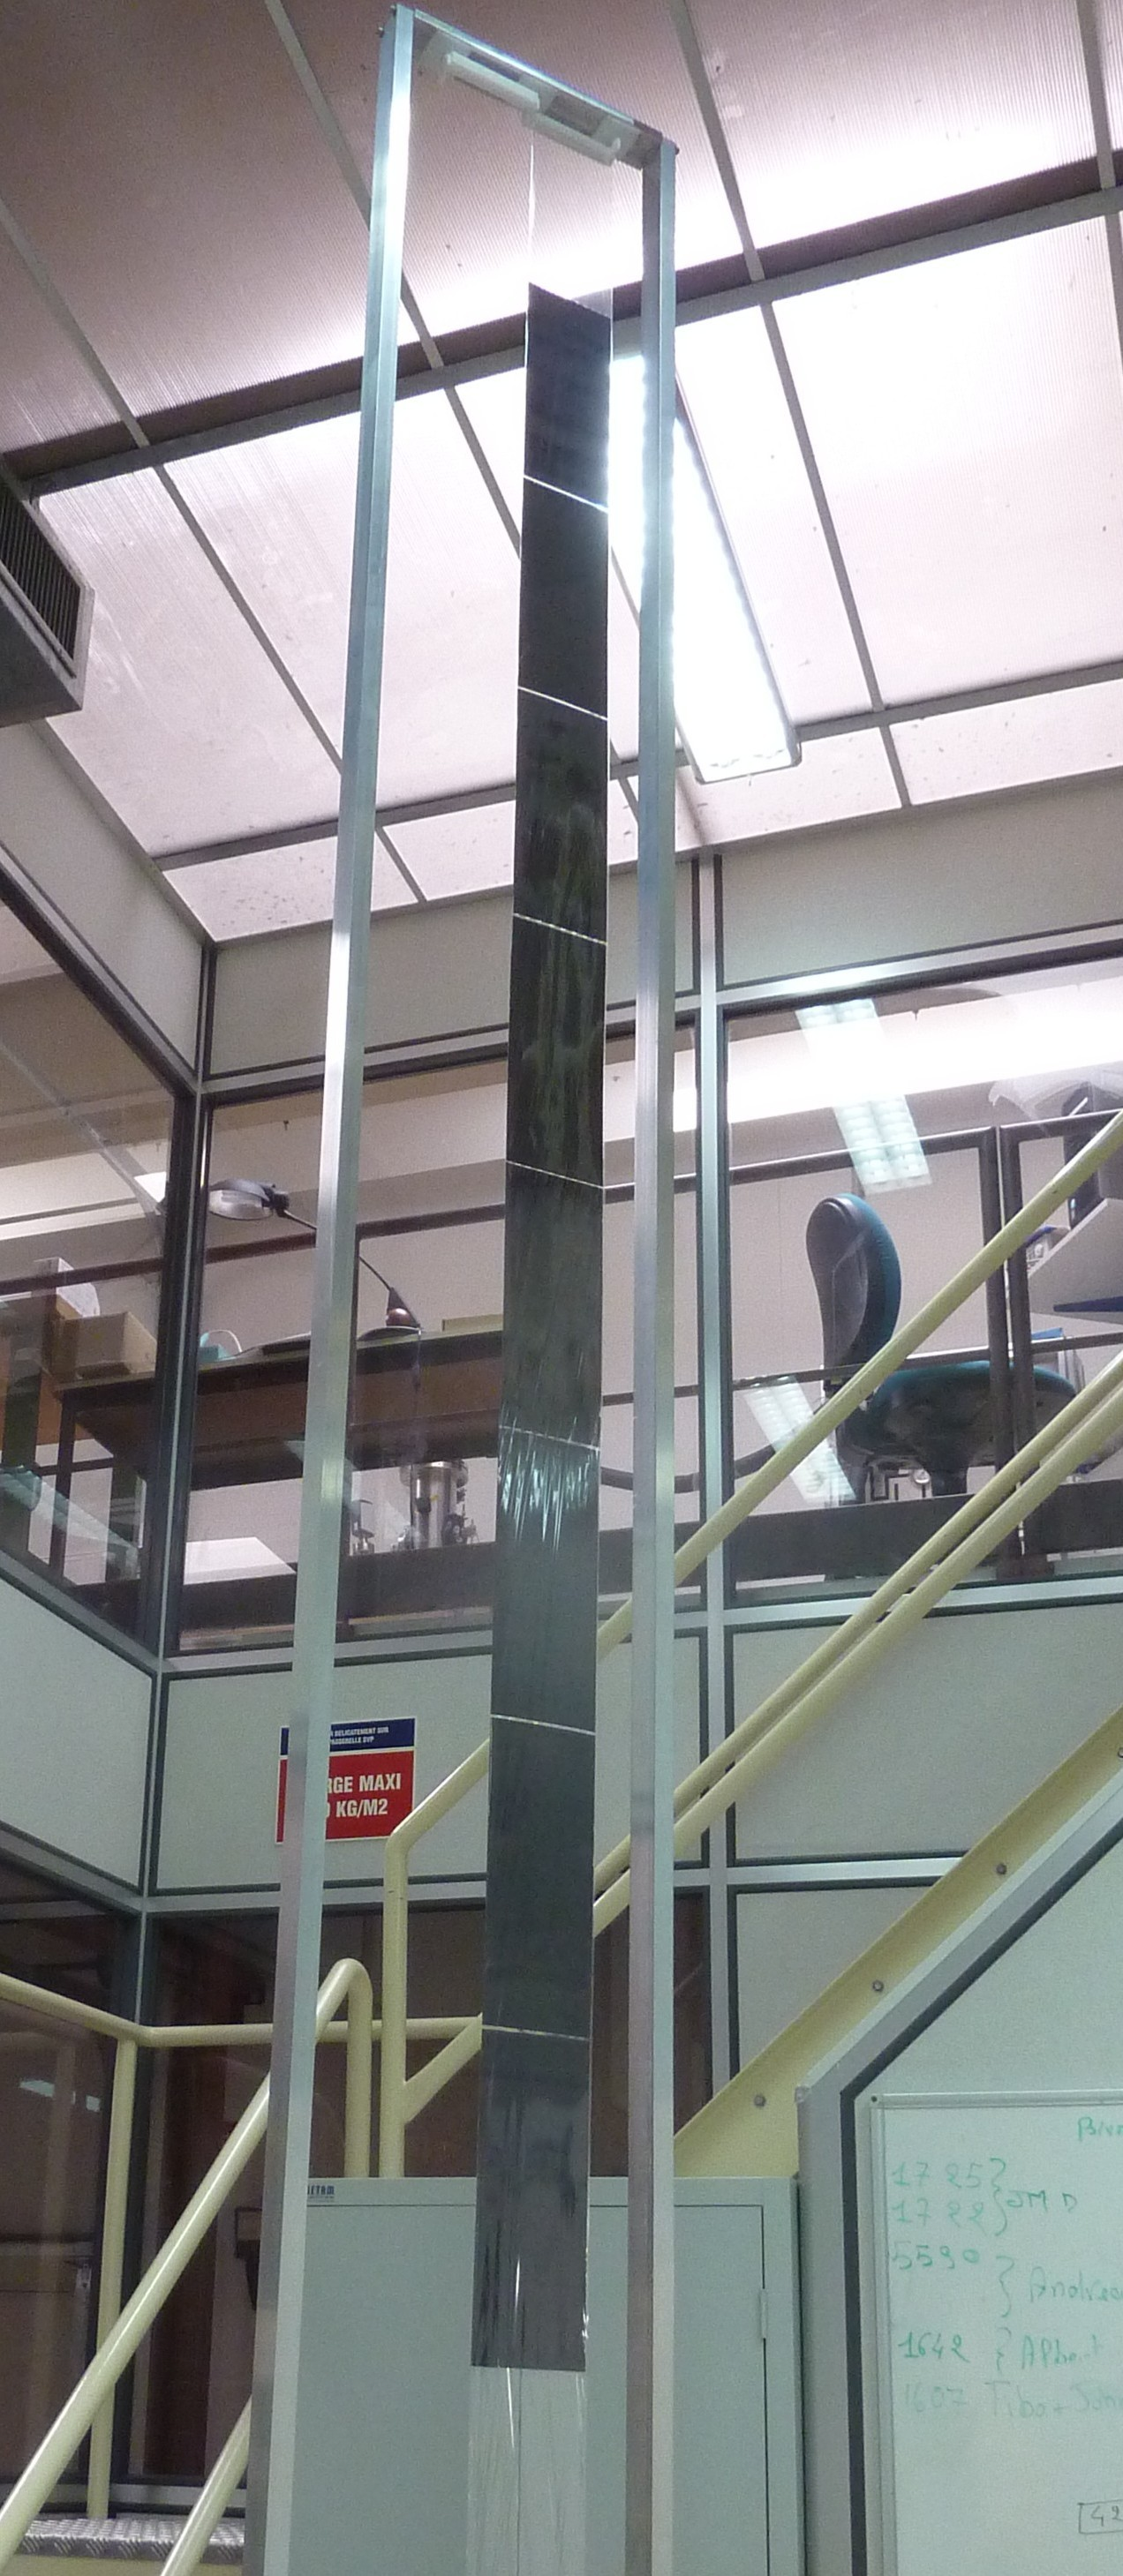
\includegraphics[scale=0.075]{pictures/Chap3/P1090162.JPG}
\caption{Left : Selenium source foils final geometry, it is divided in 36 foils
(34 with 13.55 cm width and 2 with 12.5 cm width). Right : Picture of one strip : the Se+PVA pad is surrounded by two raw mylar foils. These
two raw mylar foils are welded.} 
\label{SuperNEMOFoils}
\end{center}
\end{figure}


\NI The selenium is under a powder form. This powder is mixed with a radiopure glue (PolyVinyl Alcohol : PVA) and ultrapure water to obtain a liquid paste. This paste is spread out between two a mylar sheet of 10~$\mu$m thick pierced by micro-holes. These micro-holes allow a good coupling between the paste and the foil and facilitate evaporation. Unfortunately, these holes was made at JINR Dubna using a ions beam which can contaminate the source foil. It is in this optic that a new foil fabrication procedure have been proposed and studied in R\&D. The second method consists of unfolding the selenium foil and cut it into pads. These pads are then inserted into two mylar foils joined with a weld (mylar without micro-holes so not irradiated). More detailled on source foil optimisation will be given in Chapter~4.


\bigskip


\NI To reach a sensitivity of 10$^{\text{26}}$~years, the required level of radiopurity is 2$\mu$Bs/kg and 10$\mu$Bs/kg for $^{\text{208}}$Tl and $^{\text{214}}$Bi. The selenium must be enriched and purified. Two purification methods have been studied  : a chemical one and by distillation. 

\ifx
aa
\fi

\FloatBarrier


\subsection{The BiPo detector}


\NI The measurement of very low levels of radiopurity is not possible using germanium detector, as is generally the case. Their sensitivity is around 50 $\mu$Bq/kg for the level of $^{\text{208}}$Tl. The NEMO collaboration decided to develop and build a detector dedicated to the measurement of very low contaminations (in $^{\text{214}}$Bi and $^{\text{208}}$Tl ) of the source foils.


\bigskip  


\NI To identify $^{\text{214}}$Bi and $^{\text{208}}$Tl, the BiPo detector~\cite{BiPoDetector} is based on the observation of the so-called BiPo events. In the decay chain of $^{\text{238}}$U and $^{\text{232}}$Th, BiPo events are cascades of $\beta$ and delayed $\alpha$ decays. For example, as shown in Figure~\ref{BiPoDecayChain}, in uranium decay chain, $^{\text{214}}$Bi is a $\beta$ emitter decaying to $^{\text{214}}$Po, which is itself an $\alpha$ emitter with a characteristic half-life of 164~$\mu$s.


\begin{figure}[h!]
\begin{center}
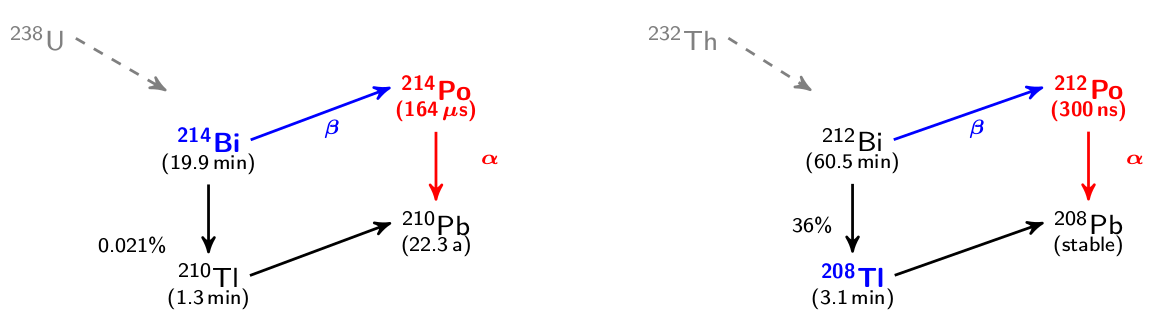
\includegraphics[scale=0.33]{pictures/Chap3/BiPoDecayChain.png}
\caption{The $^{\text{214}}$Bi$^{\text{214}}$Po and $^{\text{212}}$Bi$^{\text{212}}$Bi cascades used to measure the $^{\text{214}}$Bi and $^{\text{208}}$Tl contaminations.}
\label{BiPoDecayChain}
\end{center}
\end{figure}


\NI In order to detect the e$^-$ and $\alpha$ particles, the sources are installed between two thin ultra-radiopure plastic scintillators couplingto low radiative PMTs, as schematized in Figure~\ref{BiPoEvent}. 

\begin{figure}[h!]
\begin{center}
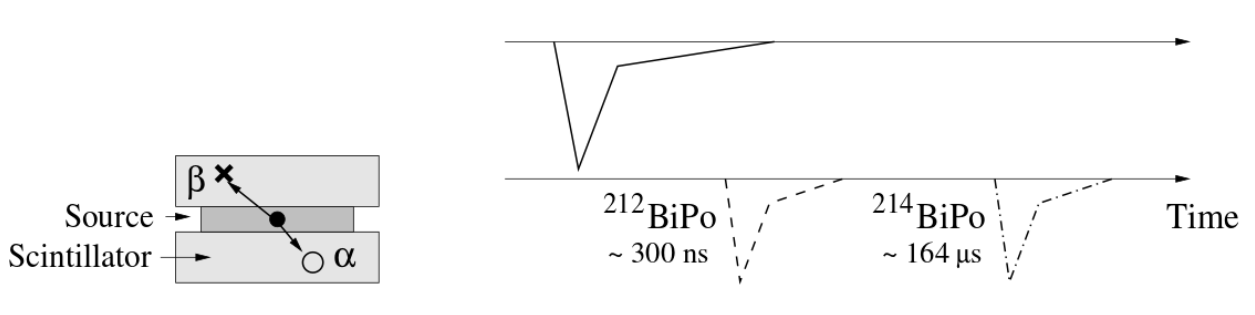
\includegraphics[scale=0.3]{pictures/Chap3/BiPoEvent_2.png}
\caption{Left : schematic view of the BiPo detection technique with the source  foil  inserted  between  two  plastic  scintillators  plate. Right : scintillation signal waveforms acquired for a BiPo event. The prompt signal  and  the  delayed signal observed  by  the  top  and  bottom scintillators respectively are schematically shown.}
\label{BiPoEvent}
\end{center}
\end{figure}


\NI The BiPo detector have been installed in 2012 at Canfranc Underground Laboratory in Spain. It is made of 2 identical modules, each of them containing 40 scintillator blocks (coupled with 5'' PMTs). Each optical module covers an aera of 30 $\times$ 30 cm$^\text{2}$, as presented in Figure~\ref{BiPoDetector}. This segmentation allows detection of possible hot spots on the foil. 


\begin{figure}[h!]
\begin{center}
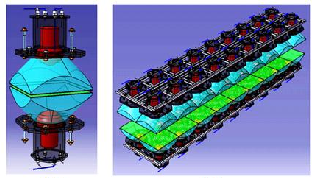
\includegraphics[scale=1.1]{pictures/Chap3/snemo_bipo.png}
\caption{Left : Pair of sub-modules coupled face to face. The green part represents the thin scintillators. The optical guides appear in blue and the PMTs in red. Right : assembly of the 40 optical sub-modules.}
\label{BiPoDetector}
\end{center}
\end{figure}


\bigskip


\NI In a first step, the detector took data without any foils to measure its own level of background. The results of 0.16~$\mu$Bq/m$^\text{2}$ in $^{\text{214}}$Bi and 1.28~$\mu$Bq/m$^\text{2}$ in $^{\text{208}}$Tl allow to reach the expected sensitivity (10 and 2~$\mu$Bq/kg in $^{\text{214}}$Bi and $^{\text{208}}$Tl) in few month of data taking.

\FloatBarrier


\subsection{Tracking volume}


\NI The tracking volume of SuperNEMO consists of 2 tracker modules made of 9 layers of 113 Geiger cells (for a total of 2034 Geiger cells). Each module is divided into 2 cassettes (for a total of 4 cassettes called C0, C1, C2 and C3) and mesure 5~m long, 3.4~m high and 40~cm depth. The tracker cells have been built and tested in Manchester before being transport at LSM.


\bigskip


\NI The commissioning of the first cassette used cosmic muon events with scintillator planes below the tracker volume 
acting as a trigger. A picture of a cassette and cosmic muon event is shown in Figure~\ref{SnemoTracker}. Of the 2034 tested cells, 23 are considered as bad (self trigger or plasma block). The proportion of operational channels is 98.9~\%. 


\bigskip


\NI During the R\&D phase a great care have been taken in order to drastically reduce the presence of radon inside the tracking volume. Based on the NEMO-3 analysis, 2 main reasons have been identified : the emanation of radon coming from the tracking device materials and a bad impermeability of the seals closing the volume (easy diffusion of the radon coming from PMTs).


\bigskip

\NI During the R\&D phase, different points have been studied to improve the wire chamber compared to NEMO-3 : 


\begin{itemize}
\item now, the wire chamber is isolated from the rest of the detector with a nylon radon-tight film.


\item Free-radon air will be introduced very close to the PMT to avoid high radon concentration. Futhermore, the entire detector will be inside a radon clean tent.


\item To maintain the tracking properties of the detector, the mixture ratio of the gas must be kept constant 
(95~\% Helium, 4~\% Ethanol and 1~\% Argon). A gas system ensures minxing and sends the gas into the detector. Great improvement have been done to purify the tracker gas. The helium can be easily purify using a coal traps.


\item all the materials placed inside the tracker volume are tested and measured in germanium detector. Emanation measurements are realized on each cassette to check that the mechanical processes have not introduced contaminations. The results of these measurements are summarized in Table~\ref{tab:RadonEmanation}. Extrapolated to full demonstrator, the value of 0.21~mBq/m$^{\text{3}}$ is obtain at nominal flowrate (0.12~mBq/m$^{\text{3}}$ when flushed at 1m$^{\text{3}}$/hr). 
\end{itemize}


\begin{figure}[h!]
\begin{center}
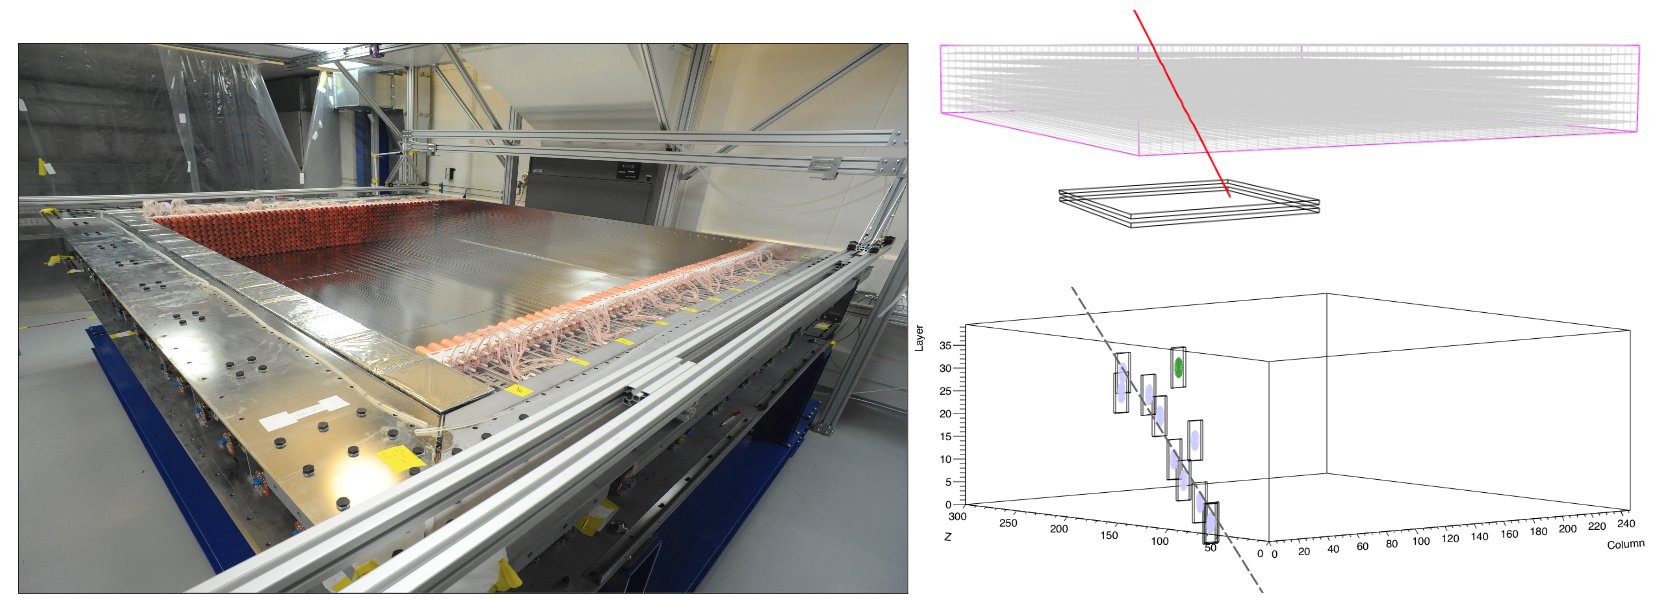
\includegraphics[scale=0.25]{pictures/Chap3/TrackerTestCosmic.png}
\caption{Left : picture of one of the four cassette fully assembled. The cassette is set horizontally, later in the SuperNEMO demonstrator, the Geiger cells will be vertical, parallel to the source foil. The copper part are the end-caps supporting the wires. Top right : simulation of a cosmic muon crossing throught the tracker. Bottom right : real event of a cosmic muon crossing the tracker.}
\label{SnemoTracker}
\end{center}
\end{figure}


\begin{table}[h!]
\centering
\begin{tabular}{c|c}
Cassette & Radon emanation \\
\toprule
C0 & 11.37 $\pm$ 1.44~mBq \\
C1 & 15.26 $^{+\text{2.5}}_{\text{4.0}}$~mBq \\
C2 & 3.28 $\pm$ 1.39~mBq \\
\bottomrule
\end{tabular}
\caption{Summary of the emanation measurements of the different cassette. The C4 have not been measured.}
\label{tab:RadonEmanation}
\end{table}


\NI The tracker volume will be coupled with a magnetic field (parallel to the source foil) for charge discrimination. Some studies have been realized to optimize its value (probably 25~G will be applied). 



\FloatBarrier

\subsection{Calorimeter}


\NI The calorimeter of the SuperNEMO demonstrator is composed of 712 optical modules distributed in 6 walls : 


\begin{itemize}

\item 2 main walls on opposite sides of the of the source foil faces. Each main wall contains 260~polystyrene cubic scintillator  blocks (256~mm $\times$ 256~mm $\times$ 194~mm) coupled to 8'' low radioactive PMT (R5912-03) which have a quantum efficiency between 35 and 45~\% at 420~nm. A main difference with the NEMO-3 blocks is that the PMT is directly coupled to the scintillator block, no light guide is used as it is shown in Figure~\ref{SnemoOpticalModule}. Thanks to this new design the energy resolution is highly improved (FWHM of 8~\% at 1~MeV).


\item 2 $\gamma$-veto to cap the top and the bottom of the detector containing 64~plastics scintillator blocks (210~mm $\times$ 200~mm $\times$ 145~mm) coupled to 5'' PMTs (R6594). 

\item 2 x-walls to cap the sides made of 32~plastics scintillator blocks (290~mm $\times$ 304~mm $\times$ 145~mm) also coupled to 5'' PMT.

\end{itemize}


\begin{figure}[h!]
\begin{center}
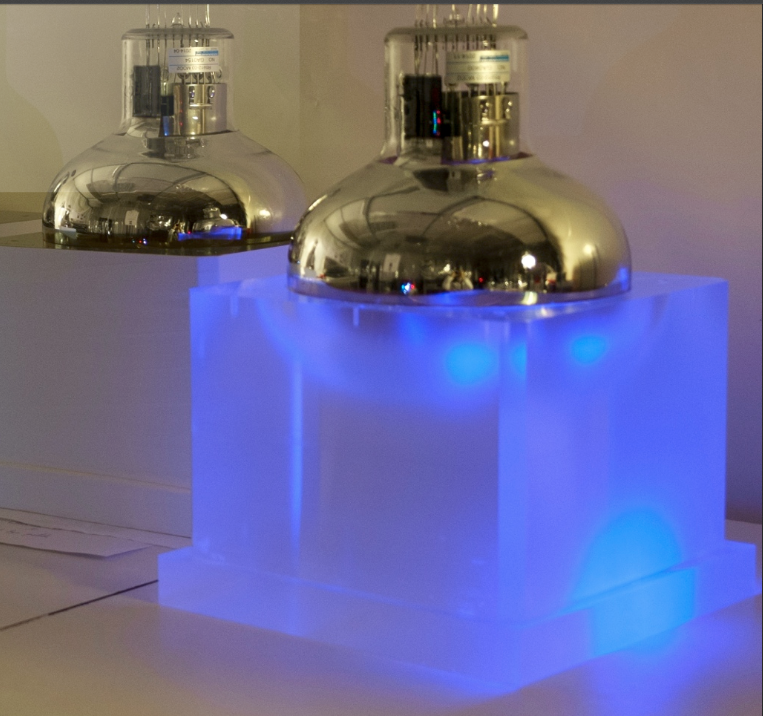
\includegraphics[scale=0.25]{pictures/Chap3/calo_1.png}
\caption{Optical module composing the calorimeter before to be wrapped into teflon and mylar. The scintillator block is directly coupled to the PMT.}
\label{SnemoOpticalModule}
\end{center}
\end{figure}


\NI To improve the light collection, all the blocks are wrapped into teflon for each block sides except the entry face which is covered by 6~$\mu$m of aluminized mylar.


\bigskip


\NI Figure~\ref{SnemoCaloFrontView} is a picture of the SuperNEMO main wall during its construction at LSM. For lack of 8'' PMTs, all the blocks in the top and bottom rows of the walls are coupled with 5'' PMTs.


\begin{figure}[h!]
\begin{center}
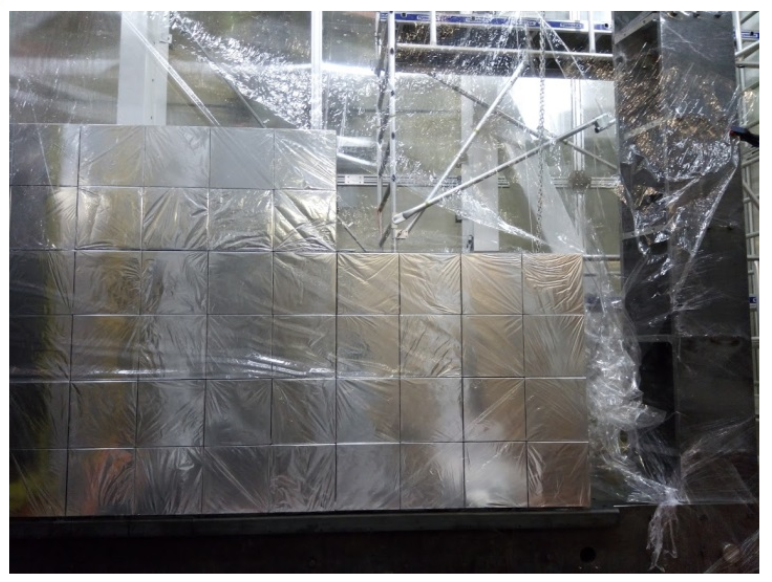
\includegraphics[scale=0.5]{pictures/Chap3/FrontViewCalo.png}
\caption{Front view of one main wall during its construction. The wall is built by assembling the bricks (8 by 8).}
\label{SnemoCaloFrontView}
\end{center}
\end{figure}

\FloatBarrier


\subsection{Calibration system}


\NI As it was the case in NEMO-3, 2 systems are used to calibrate the detector. Monthly, via a system of weights and stepper motors, $^{\text{207}}$Bi sources will be introduced inside the detector to calibrate the absolute energy scale. Between these dedicated runs, a light injection system has been developed to monitor the response and the linearity of the optical modules.


\bigskip


\NI The light injection system (LI) injects pulsed LED light into each scintillator blocks via optical fibers. A schematic view of the LI system is presented in Figure~\ref{LIschema}. Areference optical module is used to monitor the light level against a $^{\text{241}}$Am source. The 20 UV LEDs and the reference PMT are housed in a light-tight rack. The pulse height spectra recorded in a test optical module and reference block are presenter in Figure. 

\bigskip
\begin{figure}[h!]
\begin{center}
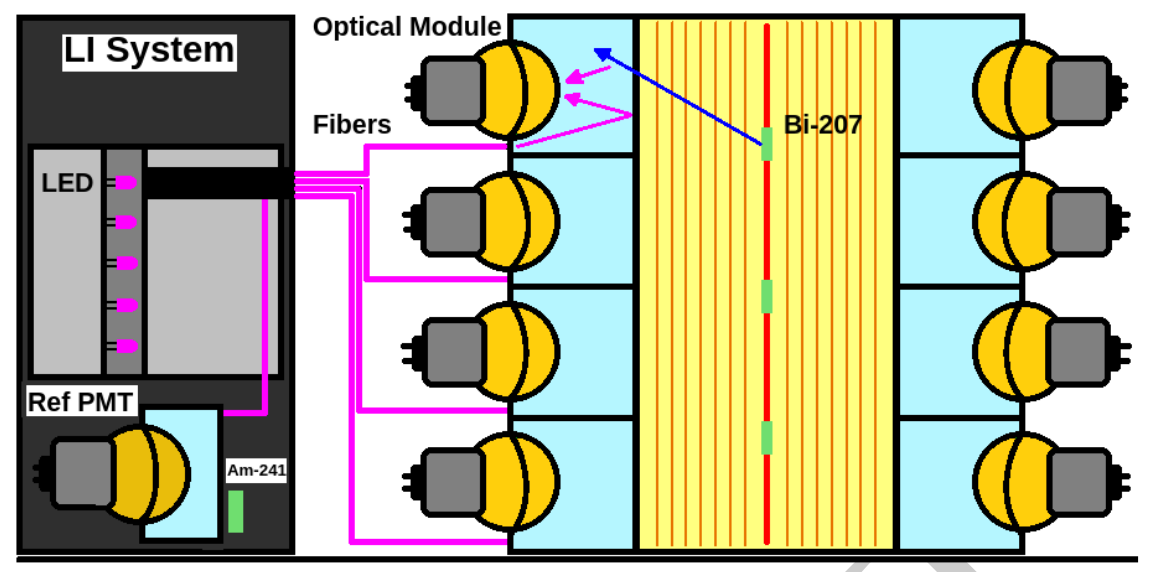
\includegraphics[scale=0.3]{pictures/Chap3/LIschema.png}
\caption{Schematic representation of the light injection system. Installed in an independant rack, a pulser will send into each optical module UV light via optical fibers. A reference PMT coupled to an americium source is used to control the light level.}
\label{LIschema}
\end{center}
\end{figure}


\NI To study how the LI system will be able to monitor and calibrate between $^{\text{207}}$Bi runs, the initial position of the 976~keV peak is used. The goal is to predict where it would be shifted to at a latter time using only the later LED peaks seen and the $^{\text{241}}$Am. Figure shows the ratio between the expected and the obserced signal, even with some jumps, the response of the optical module can be predicted within 1~\%.

\bigskip
\begin{figure}[h!]
\begin{center}
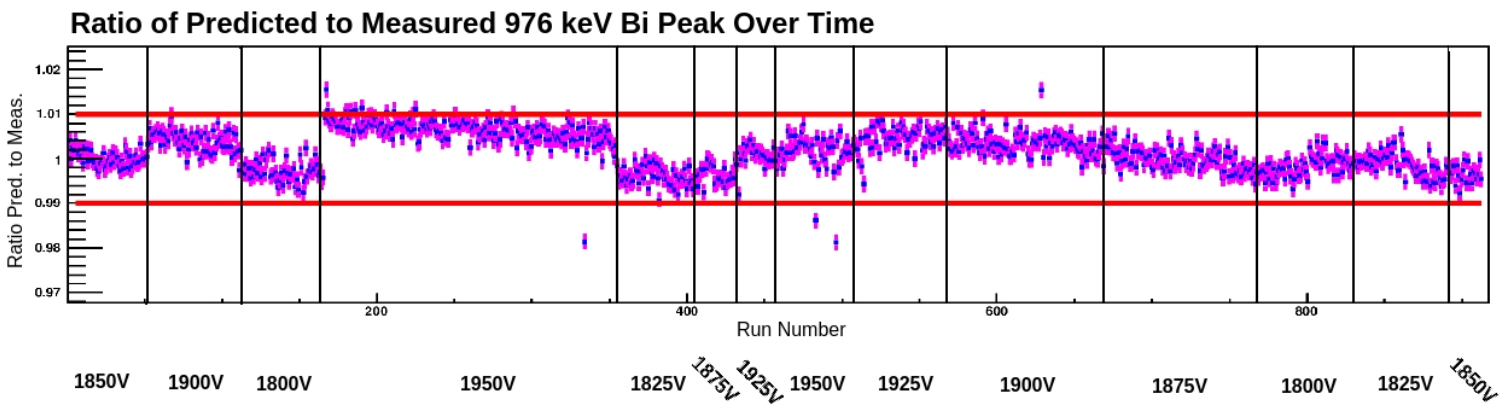
\includegraphics[scale=0.25]{pictures/Chap3/RatioPredictionLI.png}
\caption{Ratio of the predicted to measured peak position for the 976~keV $^{\text{207}}$Bi electron. The ratio deviates by not more than 1~\% as shown by the red lines.}
\label{LIschema}
\end{center}
\end{figure}


\NI In  the  LI  system,  each  LED  illumates  about  100  optical  fibers. For  linearity  tests  and  for  proper  monitoring  accuracy  the  light  receiced  for  each  optical  fibers  has  to  be  uniform. Many  studies  have  been  realized  in  the  past  to  obtain  the best  uniformity. Other problems as the light attenuation, LED optimisation or light detection are also studied. During my thesis I spent several weeks at Austin (Texas) to work on the LI system. The summary of the work I realized on it are presented in Annex~2.


\FloatBarrier


\subsection{Prospectives}

\NI \textcolor{red}{Modifier cette partie en fonction des news.}

\NI The detector is in construction phase. All the main modules (tracker and calorimeter) are at LSM. In a first phase, a calorimeter and a tracker have been joined to form a half-detector. Since the beginning of 2017, light and gas leak test are currently ongoing for an half a the detector. The source foils will be installed in .....


\bigskip


\NI In case the detector is able to demonstrate the feasibility of the experiment at large scale, the collaboration (subject to the necessary resources being made available) will build the other 19 modules. Then, the full SuperNEMO project should reach a sensitivity of 10$^{\text{26}}$~years using 100~kg of $^{\text{82}}$Se. The inital idea was to install all the module inside the new extension of the LSM laboratory. Since this new extension will not be built, the different modules could be separted over the different underground laboratory in the world. 


\end{document}
